\begin{figure}[H]
\center
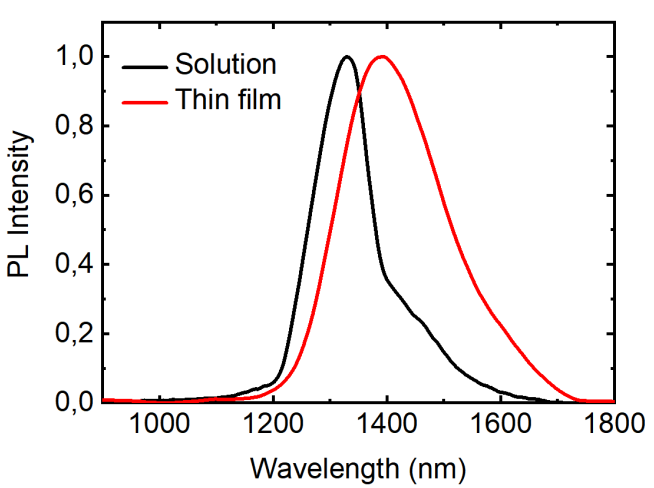
\includegraphics[width=0.7\textwidth]{ch5/Pbs-QDs1st_emm}
\caption{Emission spectrum of used PbS QDs \cite{2011}}
\end{figure}

The whole idea of all-solution processed QD solar cells is beginning to mark its footprint in modern photovoltaics. Within all of type III SC PbS QDs are promising candidates and certainly a field of quick improvement. Yet, what is so promising about them and what are the features that distinguish them from other types. 
In case of PbS QDs it must be denoted that the main advantages that they provide are the high efficiency and wide bandgap tunability due to its direct link with quantum dot size. For photovoltaic purposes the next important thing would be the ability to multiple excitation through the band gap. 

They are used in many different structured solar cells, creating a numerous variations of junctions and quantum dot treatments and achieved over 11\% power PCE as for last few years. The main problems with them would be to conduct and choose a fine ligand passivation. In our case the halide anions from precursors of tetrabutylammonium iodide (TBAI) and 1,2-ethanedithiol (EDT) were used. Ligands from such precursors do not only, more or less precisely, passivate surface defects, which are of course unsatisfactory for our case, but modify electronic properties of QDs as well. The PbS-EDT layer was used as hole transport and  PbS-TBAI, a main light harvesting layer,  has been reported to usually be a n-type semiconductor, probably owing to a) $I^{-}$  anions that are exchanged in PbS QDS with $S_2^{-}$ and b) $I^{-}$ anions are bound to the surface and repulse a oxidative processes. The choice of those were due to rather improved stability of QDs comparing to other layer passivating (devices with TBAI and EDT bi-ligands have been shown to provide a much longer stability in air than others). Although a longer air-exposure provides undesirable consequences that downgrade the cell significantly, the short period exposure is suspected of creating a more efficient charge extraction. Nevertheless, the inner processes that allow that bi-layer structure to be one of the best, provided for those types of QDSCs, is still eluded and further improvements are expected if it becomes much more understood. For example, a greatly simplified deposition has been achieved by replacing methanol with acetonitrile, which consequently improved electrical properties of photovoltaic device as well. (The device structure was very similar to ours). There are irrefutable results in achieving fine results from synthetisation from the group\cite{Wang2017} \cite{Hu2016}.

\subsection{$\mathbf{PbS}$ Quantum Dots produced in our laboratory}

\begin{figure}
\centering
\begin{subfigure}[b]{0.7\textwidth}
\centering
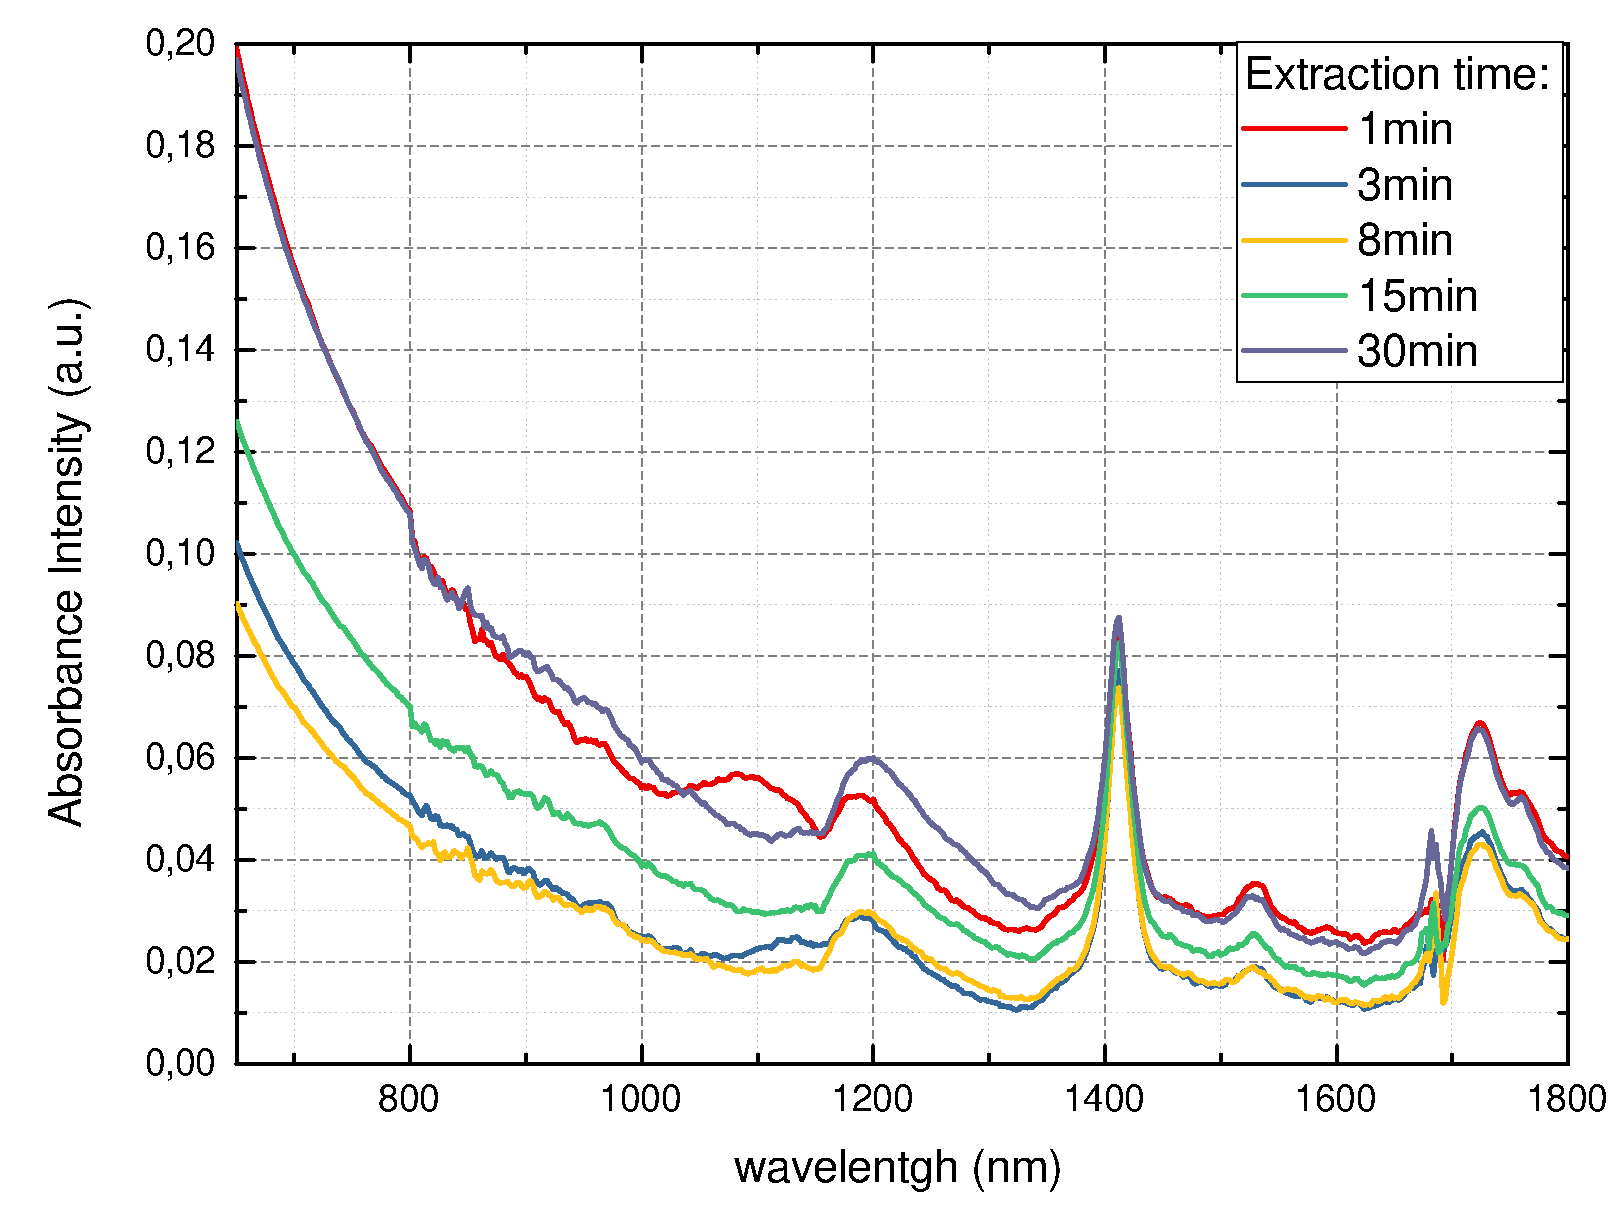
\includegraphics[width = \textwidth]{ch5/synth/Abs002}
\caption{Absorbtion spectrum}
\end{subfigure}

\hfill

\begin{subfigure}[b]{0.7\textwidth}
\centering
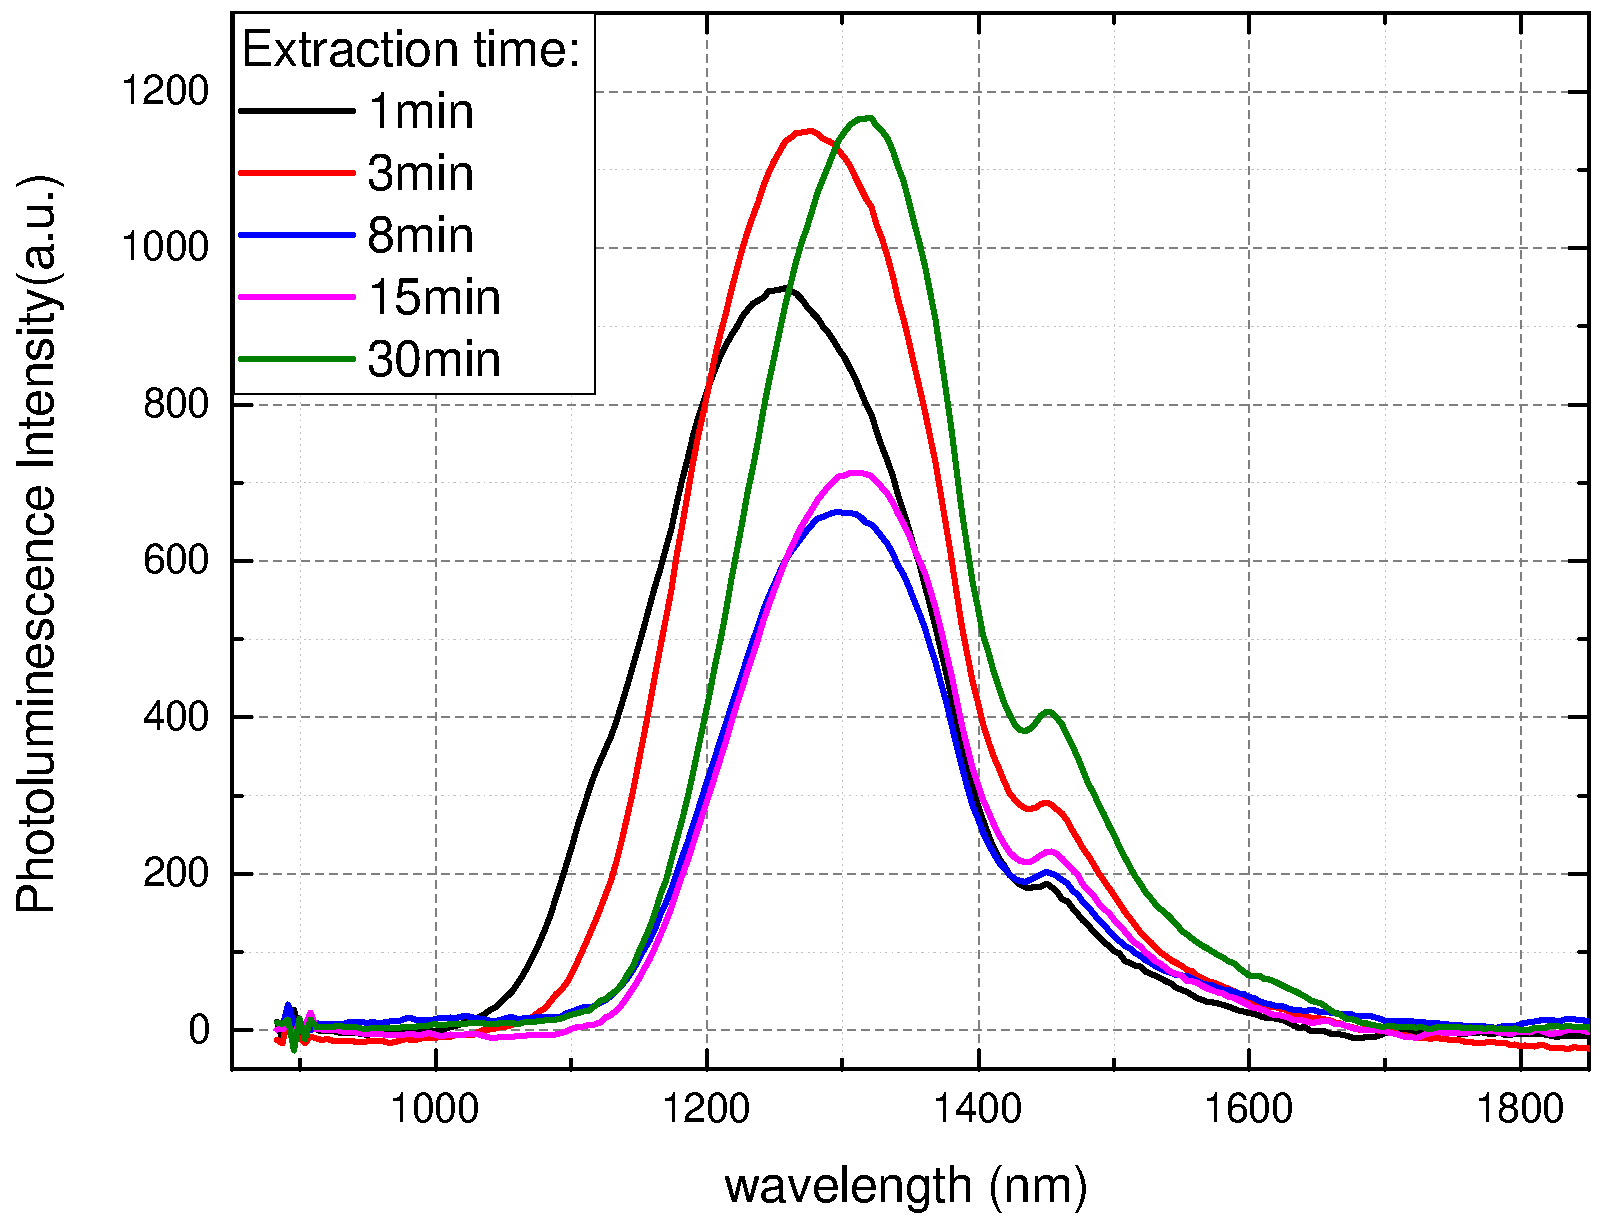
\includegraphics[width = \textwidth]{ch5/synth/PL002}
\caption{Photoluminescence spectrum}
\label{fig:synth}
\end{subfigure}

\caption{Optical measurements of QDs synthesized by \cite{swietek} and the procedure is described right there. It is worth to mention that the injection has been made at 80$\deg C$. Graphs were included with kind acceptance of the former thesis author}
\end{figure}

The manufacture of CQDs is an effect of cooperation between the group members, and the results in the synthesis of PbS Quantum Dots are ought to them. Those nanostructures are similar from time to time, yet being improved with each synthesis. We will discuss the effects shortly but more can be found in \cite{swietek}, which is a complementary thesis to this one, done by a student from the group. We can see that the width in luminescence spectrum isn't yet sufficient, as we would like to reabsorb only small amount of the photons to reduce phononic effects, but it's getting much better. Also, the absorbtion spectrum is really impressive with few peaks overlapping with solar spectra, as we would like to extract electrons where the intensity is the highest. (Fig.\ref{fig:synth}) 


\subsection{First device deposition}

A first insight of what can we do and what would be the challenges to overcome has been made due to creation of a first working solar cell. The cell was based on PbS QDs and it has shown a promising quantities for further development. The whole subchapter provides a comparison of Vimun SC-3514 $3^{rd}$ generation silicon solar cell and our own QDSC.


\subsubsection{Device fabrication}
The support for a whole device was ITO-coated glass substrate that was cleaned with strong solvents and drained ultrasonically. After that a double layer of ZnO was created by using a spin-coater and after annealing PbS QDs were fabricated using spin-coating as well. It is important to denote, that it was possible to create a multi-deposition layers of QDs, which means the structure isn’t eluted from the ground. The layers were successfully dried in vacuum. After that, a $MoO_x$ firm has been added for creating inside trapping states and with sputtering process Al contacts were created on the device. As many heavy-metal QD semiconductors are toxic and degrade in air they must be also encapsulated in a stable polymer shell to avoid exposure. 

\begin{figure}[H]
\center
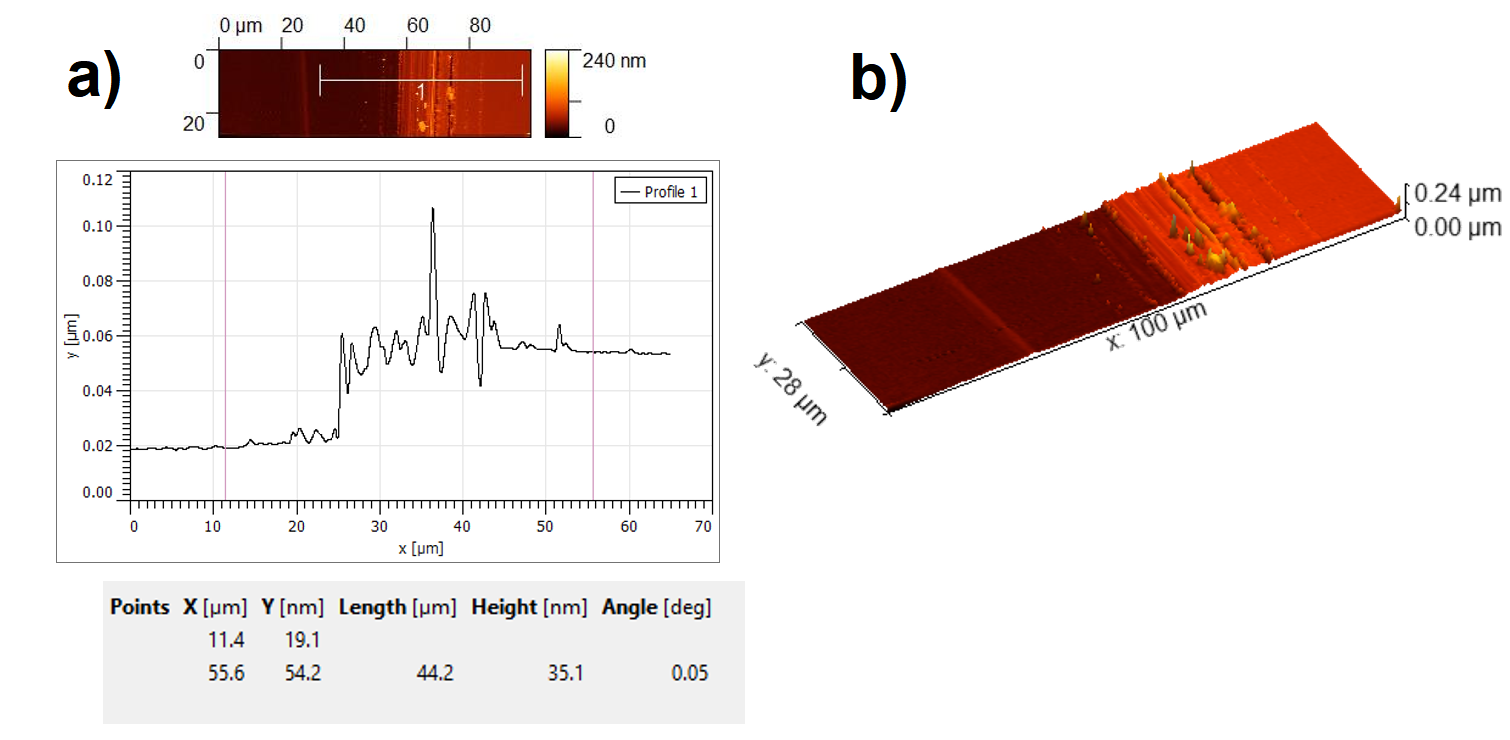
\includegraphics[width=\textwidth]{ch5/afm}
\caption{AFM picture of deposited ZnMgO layer. It has been done on the ITO glass contact. We can clearly see the border between two materials. The width of the layer is estimated to be 0,04$\mu m$ taking the average line.}
\end{figure}

\begin{figure}
\center
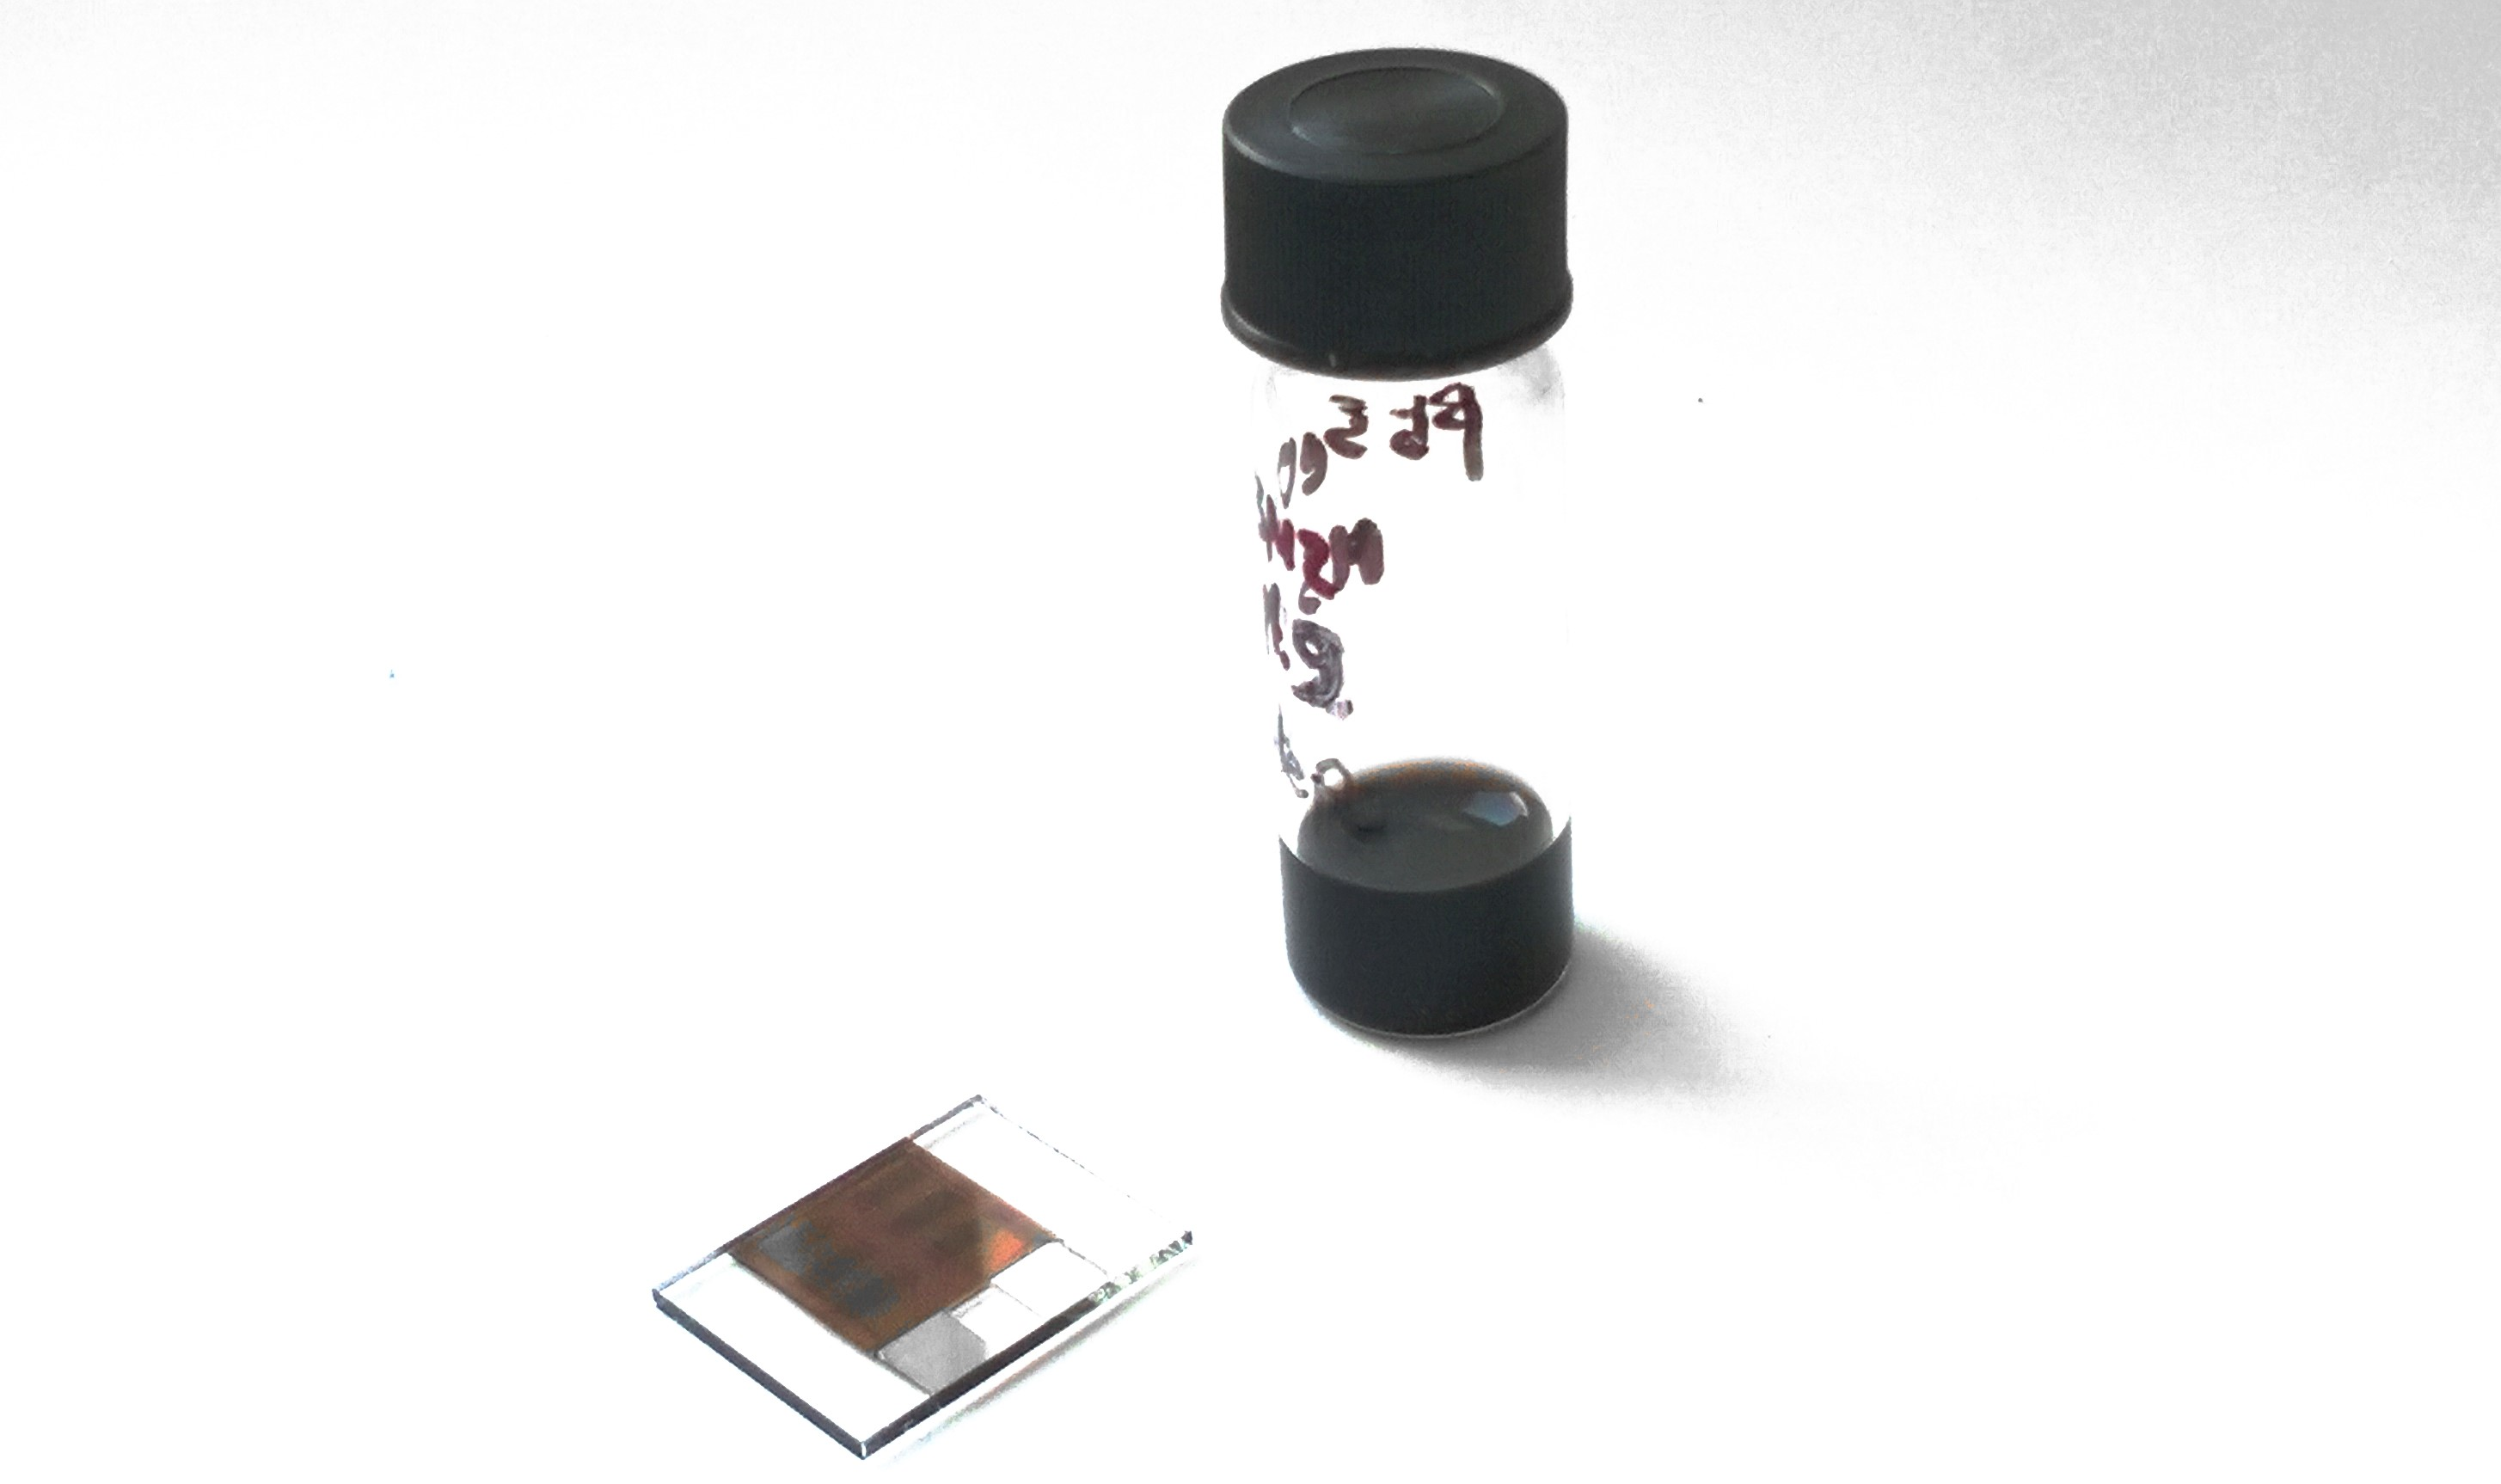
\includegraphics[width=0.75\textwidth]{ch5/IstSC}
\caption{First device and PbS Quantum-Dots produced in our lab}
\end{figure}

\newpage
\subsubsection{Results}

From the following calculations we were able to compare both of the solar cells to distinguish what shall be definitely improved to achieve better effects. Standard photovoltaic measurements were provided to create IV both IV characteristics. However, it has to be denoted that neither were the surfaces of both devices the same, nor were the lengths from the light source. 

\begin{figure}[H]
\center
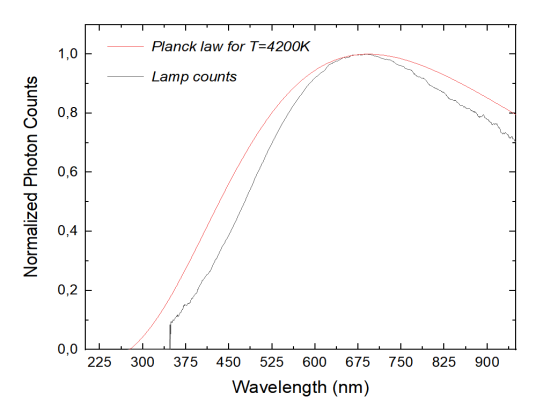
\includegraphics[width=0.81\textwidth]{ch5/bb1stco}
\caption{Comparison of Black Body photon counts and that of our light source}
\end{figure}

Therefore a certain calculations and assumptions were made. From the
photo-diode detector which were illuminated from the light source from
\(h_{d} = 400mm\) we calculate the \(P_{d}\)-power on the detector. We know that the photo-diode responsivity: \\ \\ \\ \\ 

\begin{equation}
R_{\lambda} = \frac{I_{p}}{P} = \frac{I_{p}}{r_{p} \cdot \frac{\text{hc}}{\lambda}}
\end{equation}

where \(I_{p}\) is a photo-current output, and P is a ratio of radiant
energy incident on the photodiode, which directly enables to calculate
\(r_{p} -\) photon flux(number of photons/sec). We also define quantum
efficiency of a photodetector as:
\begin{equation}
\eta = \frac{r_{e}}{r_{p}}
\end{equation}


\noindent which is the number of light created electrons to number of incident
photons. That depends on wavelength through absorption coefficient,
thickness of layers etc. Therefore we can say that:

\begin{equation}
r_{e} = \eta r_{p} = \frac{\eta P}{\frac{hc}{\lambda}} \rightarrow I_{p} = \frac{e\eta P}{\frac{hc}{\lambda}}
\end{equation}


 Therefore, responsivity may be written as:

\begin{equation}
R_{\lambda} = \frac{e\eta P}{hc}
\end{equation}


 According to those calculations we now see that from:
\begin{equation}
J_{sc} = e\int_{\lambda}^{}{\Phi_{p}(\lambda ) \cdot \eta (\lambda) d \lambda }
\end{equation}

 \(\Phi_{p} -\) is a photon flux now, for the sake of new calculations to
distinguish the difference of photon counts and J­\textsubscript{sc} is
a short-circuit current. From that of above we now can see that:
\begin{equation}
J_{\text{sc}} = \int_{\lambda}^{}{\Phi_{p}\left( \lambda \right) \cdot R_{\lambda } \cdot \frac{\text{hc}}{\lambda }d\lambda } \rightarrow
\end{equation}

\begin{equation}
J_{\text{sc}}^{\text{rel}} = \int_{\lambda}^{}{\Phi_{p}^{\text{norm}}\left( \lambda \right) \cdot R_{\lambda} \cdot \frac{\text{hc}}{\lambda}d\lambda }
\end{equation}


 where we have used relative value for short-circuit thanks to using a
normalised values because of the fact that detector isn't ideal and that
we can calculate the number of incident photons by simply using:
\begin{equation}
N_{p} = \frac{J_{sc}}{J_{sc}^{rel}}
\end{equation}

 From now we can clearly say that:
\begin{equation}
P_{d} = \int_{\lambda}^{}{\Phi_{p}^{\text{norm}}\left( \lambda \right) \cdot N_{p} \cdot \frac{\text{hc}}{\lambda}d \lambda }
\end{equation}

\begin{figure}[H]
\center
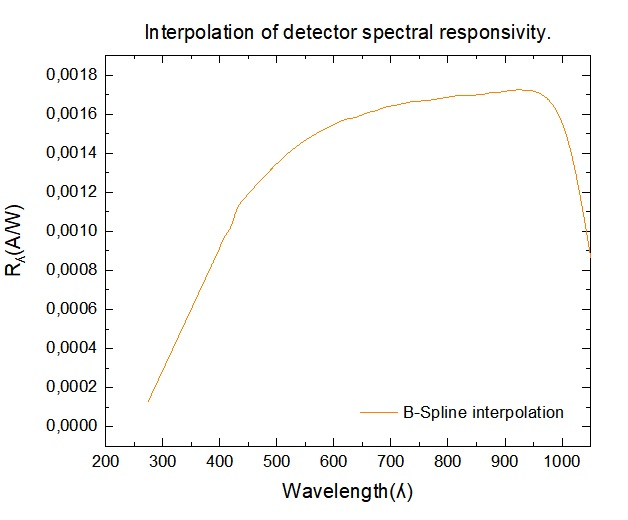
\includegraphics[width=0.8\textwidth]{ch5/GHZOPT}
\caption{Original data from Gigahertz Optik Gmbh}
\end{figure}

 From integration and minding that
\(J_{\text{sc}} = 3,5 \cdot 10^{- 4}\text{mA\ }\)we achieved that:

\[N_{p} \approx 1,4 \cdot 10^{21}\]

\[P_{d} \approx 2,71 \cdot 10^{-4} \left( W \right)\ \]

 The calculations are roughly approximated and are just a
presentation of methods used, mainly due to the fact that the full
spectral characteristics weren't absolutely known. We can now estimate
\(P_{\text{density}} \approx \frac{P}{\Omega},\) where \(\Omega\) is a
solid angle. Therefore in our case from the information from \ref{tab:1stparam} we can calculate PCEs of both
photovoltaic devices by using:
\begin{figure}[b]
	\centering
	\begin{subfigure}[b]{0.49\textwidth}
	\centering
	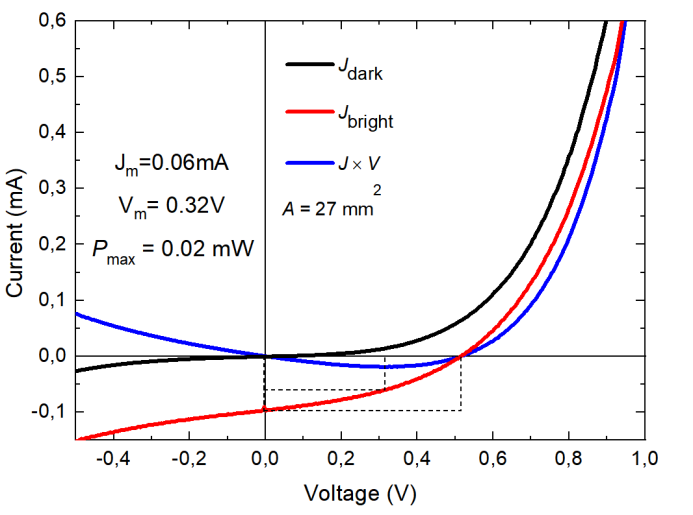
\includegraphics[width=0.93\textwidth]{ch5/istQDiv}
	\caption{QDSC}
	\end{subfigure}
	\hfill
	\begin{subfigure}[b]{0.49\textwidth}
	\centering
	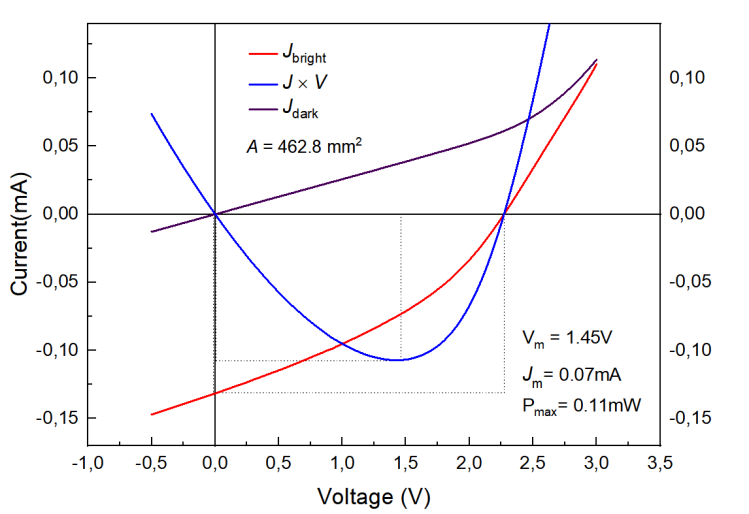
\includegraphics[width=\textwidth]{ch5/istVIMiv}
	\caption{Commercial solar cell}{}
	\end{subfigure}
	\caption{IV characteristics for QDSC and commercial cell }
\end{figure}

\begin{table}[ht]
\centering
\begin{tabular}{|c |c | c | c |}
\hline
& Detector & QDSC & Commercial Cell\\
\hline
Length from light source{[}mm{]} & 400 & 75 & 603\\
\hline
Surface{[}mm\textsuperscript{2}{]} & 36,32 & 27 & 462,8\\
\hline
Solid angle{[}sr{]} & 2,27E-04 & 4,80E-03 & 1,27E-03\\
\hline
Incident Power {[}W{]} & 2,72E-01 & 2,02E-03 & 3,47E-03\\
\hline
\end{tabular}
\caption{Parameters of tested solar cells}
\label{tab:1stparam}
\end{table}

\begin{equation}
PCE = \frac{V_{m}J_{m}}{P_{\text{in}}}
\end{equation}

\begin{table}[ht]
\centering
\begin{tabular}{|c |c |c | c | c|}
\hline
& V\textsubscript{m}{[}V{]} & I\textsubscript{m}{[}A{]} &P\textsubscript{in}{[}W{]} & PCE\\
\hline
QDSC & 0,32 & 6E-05 & 5,75E-03 & 0,33$\%$\\
\hline
Commercial Cell & 1,45 & 7E-05 & 1,53E-03 & 6,65$\%$\\
\hline
\end{tabular}
\caption{PCEs of photovoltaic devices}
\label{tab:1stPCE}
\end{table}
Provided that producer of the Commercial Cell provides similar PCE
compared to the given in \ref{tab:1stPCE} and the efficiency of our light
source is aimed to be close to 10\%, and therefore its power is 150W we
get circa 15W of light which we get by multiplying the power on the
detector by a factor of $4\pi /\Omega $ , where $\Omega$ is the solid angle for the
detector. This means that our, certainly course, calculations show
reasonable results from which we can definitely draw some conclusions.

\subsubsection{Improvements for the future prospects}

As we can clearly see, the PCE of QDSC made is small compared to the
current world efficiencies \cite{Kamat2018}. This can be caused by numerous reasons.
Working with colloidal quantum dots is always connected with the careful
arrangements of various parameters. The slightest change of just one may
provide a drastic change in the final result. Therefore we may conclude
that the reason of such an efficiency is mostly challenged by the
optimal choice of the layer width, quick degradation of QDs in the
presence of air or physical defects on the device structure. The large
leakage current may suggest that there are many defects inside the
device structure which simply create traps for moving electrons.
Nevertheless, the prospect of creating competitive QDSC is definitely in
our reach. For example, we can see that I\textsubscript{sc} is really
more than satisfactory for device with such a small surface. Now, we have to deal with
the improvement of our device. Optimization of the layer width and
enlarging of CQDs stability will be the first things to do, but
certainly not last. After testing those aspects, we may check if there
is another way to exchange ligands in CQDs, which may provide major
improvement in mobility, if there is growth of efficiency when changing
or adding another transport layer in the device structure or if layer
homogeneity can be further increased to stay comprehensive and
competitive.

\begin{figure}
\centering
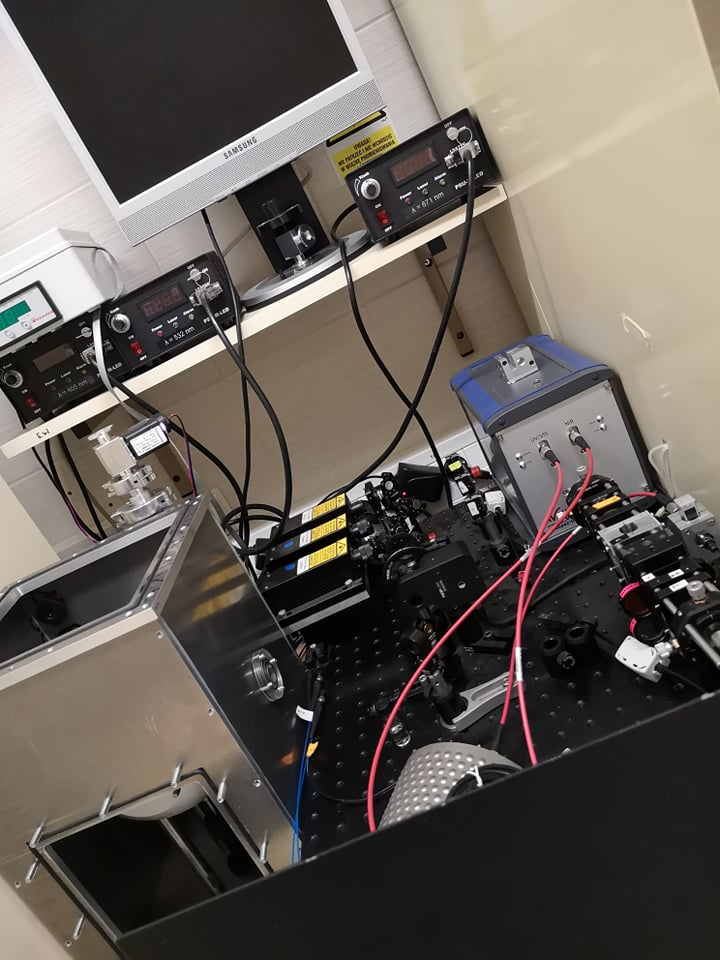
\includegraphics[width = 0.5\textwidth]{ch5/spectra_schem}
\caption{Laboratory absorption and photoluminescence measuring system }
\label{fig:pomiary}
\end{figure}
\newpage

\subsection{Second device manufacture}

The first idea was to use different layers than previously. There were great quality PbSe QDs available. From that, we have made a similar device based on those QDs. Unfortunately, the outcome of the try was unfortunate and the device wasn't able to produce any current at all. Probably it was due to mismatch between the layers and poor layer deposition. 

\begin{figure}[H]
\center
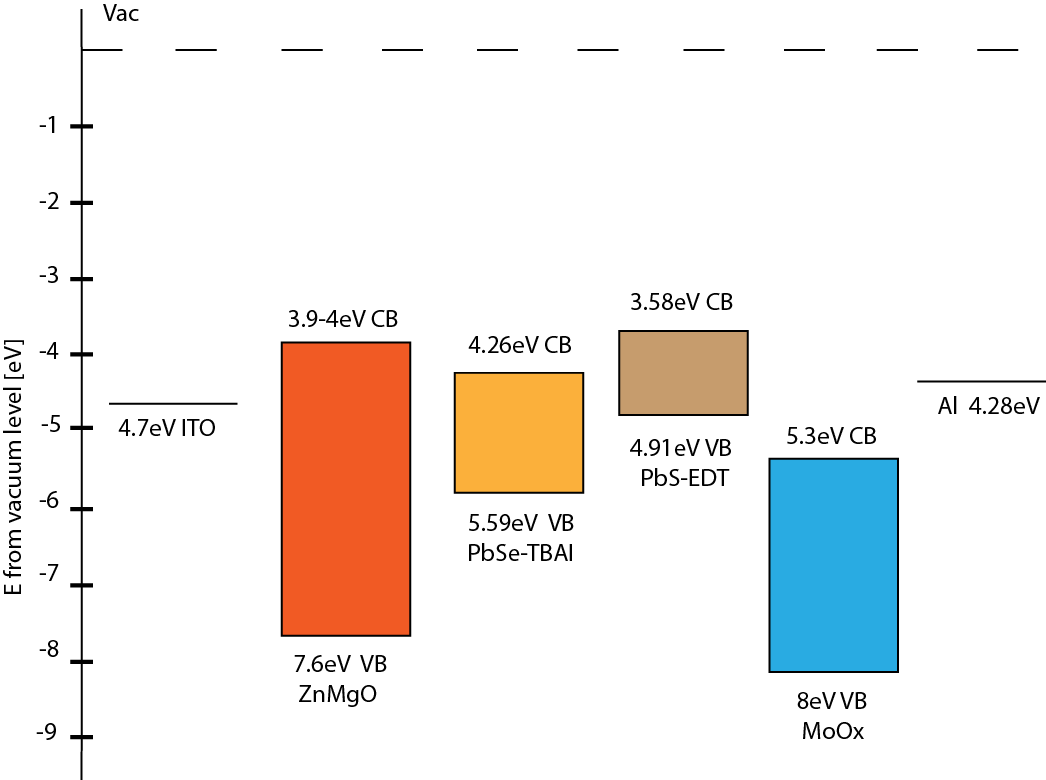
\includegraphics[width=0.9\textwidth]{ch5/STRUCTURE}
\caption{Energy structure of the first PbS-based QDSC}
\label{fig:1stEnergy}
\end{figure}

After that the second attempt of the same structure with PbS QDs was made, this time with bigger attention to fine deposition and shortened exposure to the air. Schematic of the device is very similar to it's former, except that the ZnO has been doped with Mg creating a layer of ZnMgO. However, we have used much different layer deposition times, which of course resulted in various layers width. This time also, the number of depositions was increased, also for EDT one. The purification method, which was used, has been described in Subsection(\ref{subsection:CHXpurification}) - using CHX/Acetonitrile. Later, we have achieved QDs with spectrum shown in (Fig.\ref{fig:PBS}). All the spectra have been created using the system shown in (Fig.\ref{fig:pomiary}).

\begin{figure}[H]
\centering
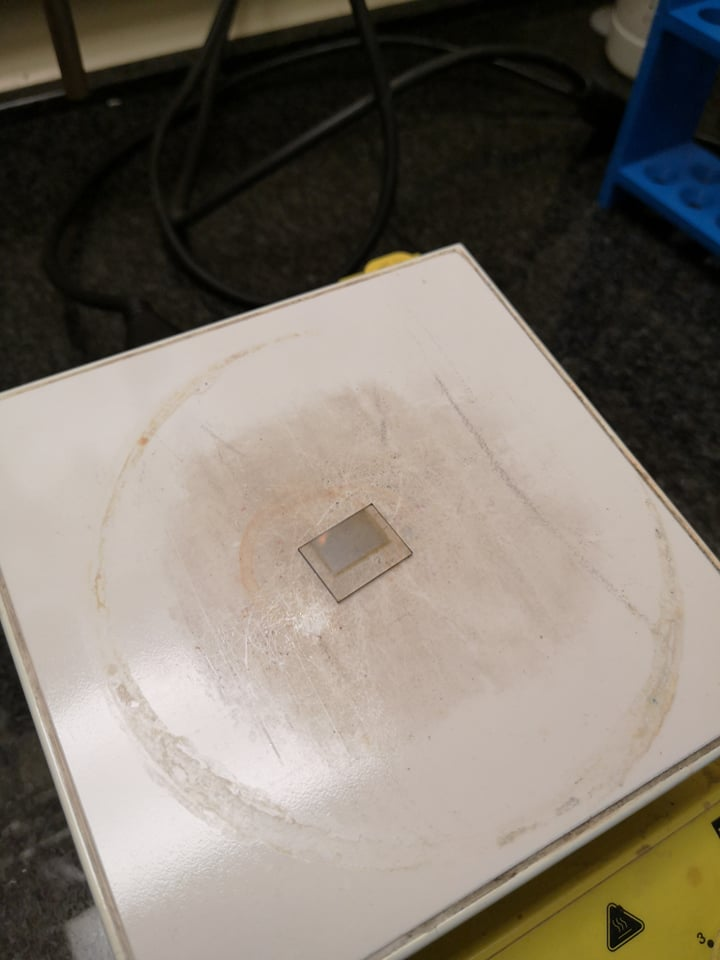
\includegraphics[width = 0.55\textwidth]{ch5/wygrzewa}
\caption{Cell heating}
\end{figure}

\begin{figure}
\center
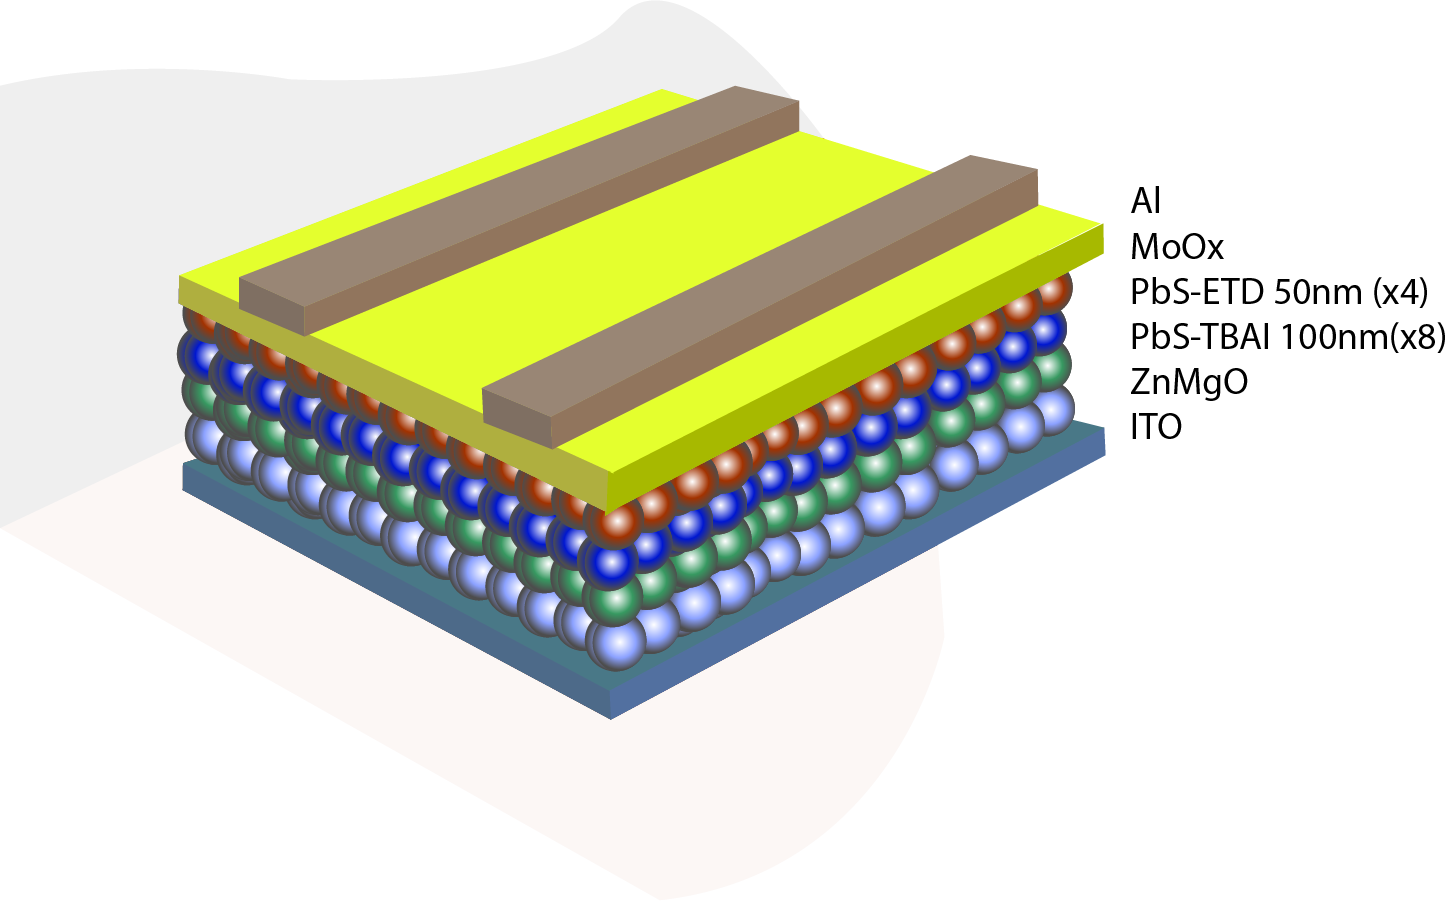
\includegraphics[width=0.9\textwidth]{ch5/3DStruct}
\caption{3D structure of the first device based on PbS QDs}
\label{fig:1stStructure}
\end{figure}
The layers were deployed using the spin-coater using this recipe from Fig. (\ref{fig:steps1}). After that, the last layer of MoOx has been deposited in the glove-box and the cell was heated to get rid of solvents and, with it, some unwanted molecules. Then, with the last electrode has been deposited using the method described in the former chapter. Again the standard photovoltaic measurements were made.

\begin{figure}
\centering
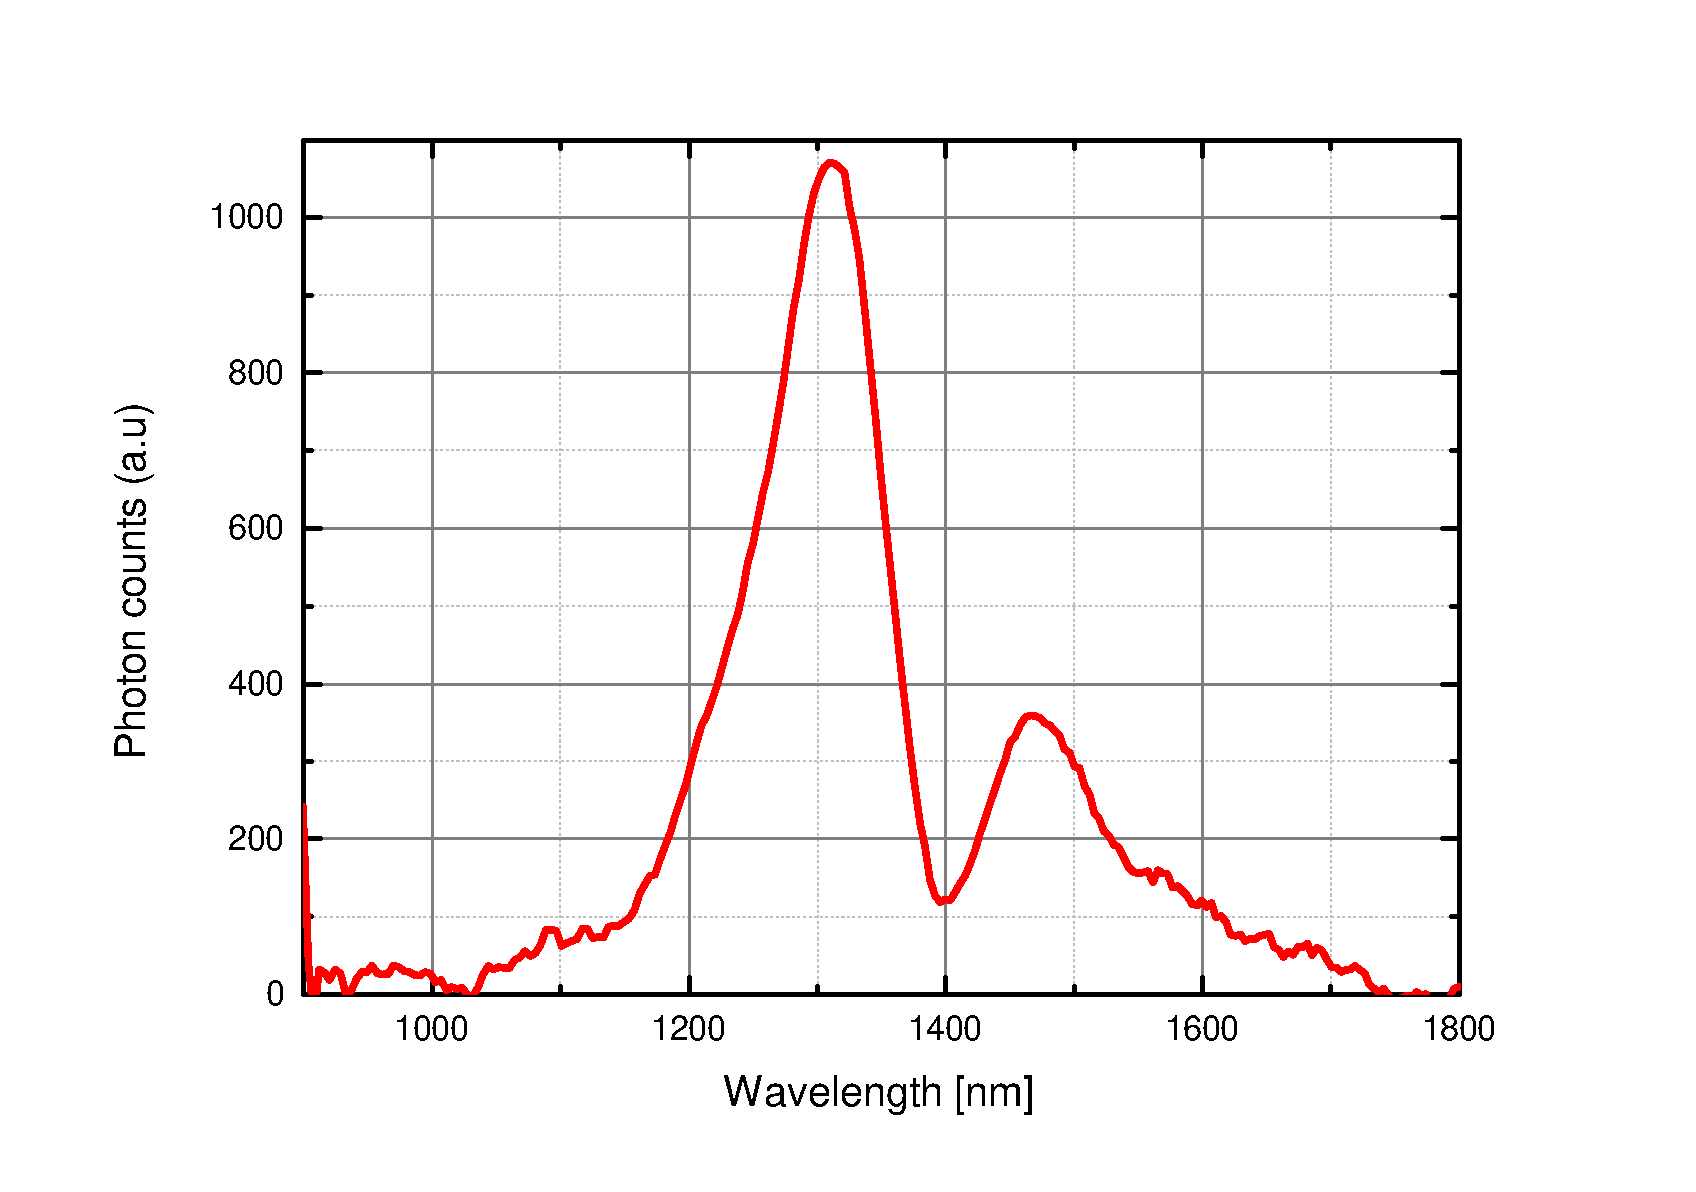
\includegraphics[width = 0.9\textwidth]{ch5/PBS-lumi}
\caption{Photoluminescence of purified QDs. Althought they aren't perfect in the subject of the width of the peak and two distinct peaks, the greater peak is placed at suitable wavelength. Those were the only PbS QDs available at the time as well. }
\label{fig:PBS}
\end{figure}


\begin{figure}[H]
\centering
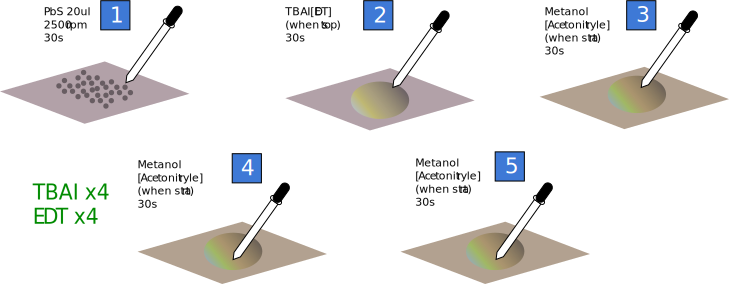
\includegraphics[width = \textwidth]{ch5/steps1}
\caption{Second deposition parameters and number of depositions made}
\label{fig:steps1}
\end{figure}

Firstly, the standard IV dark spectrum procedure has shown a quite promising characteristics(Fig.\ref{fig:firstever}). We can see, that there is a fine forward bias for the device, starting at $V_{bi} \approx 1V$. Nevertheless, the reverse bias shows an early beginning of a breakdown, which we have not expected. Probably, irreversible changes have been made to the device due to the reverse current and we will later see their effects.  

\begin{figure}
\centering
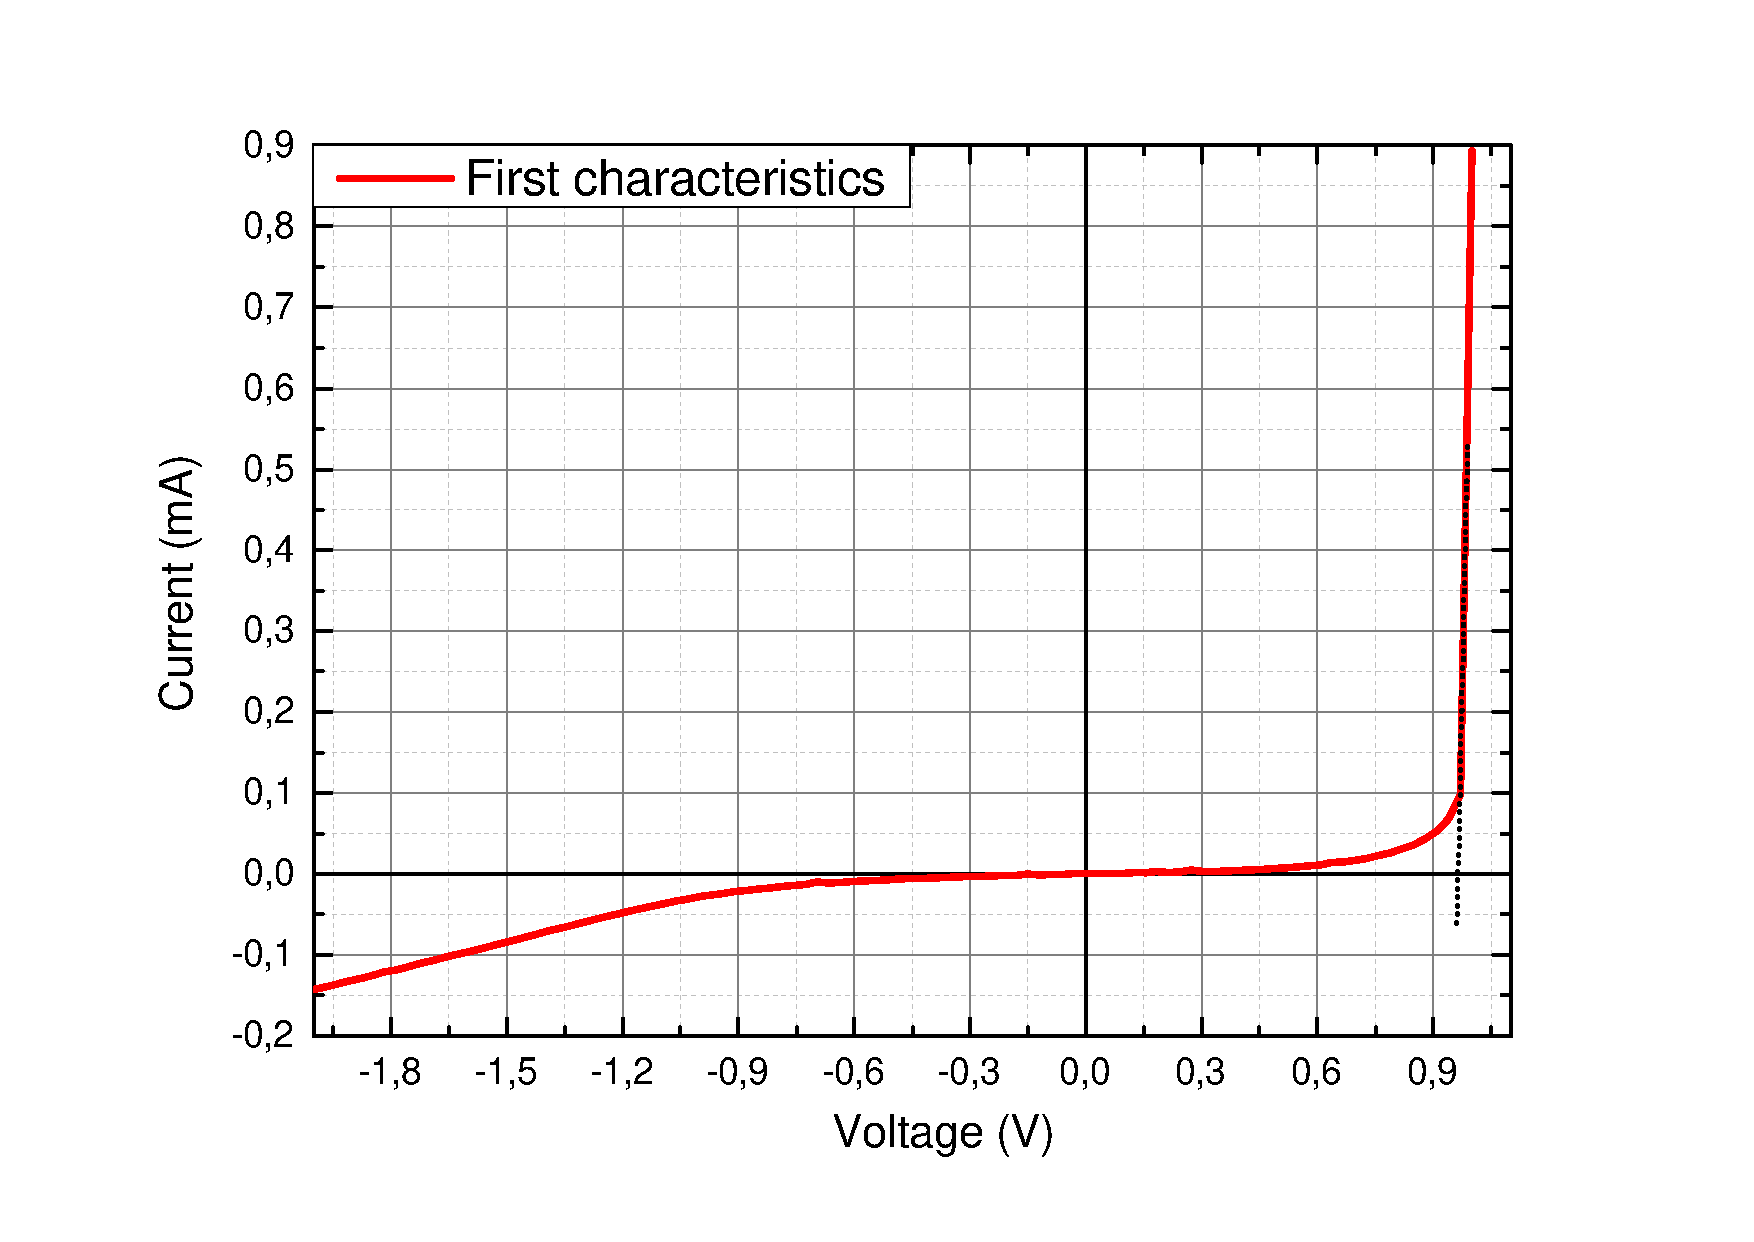
\includegraphics[width = 0.9\textwidth]{ch5/First ever}
\caption{First results from dark IV characteristics}
\label{fig:firstever}
\end{figure}

\begin{figure}
\centering
\begin{subfigure}[b]{0.83\textwidth}
\centering
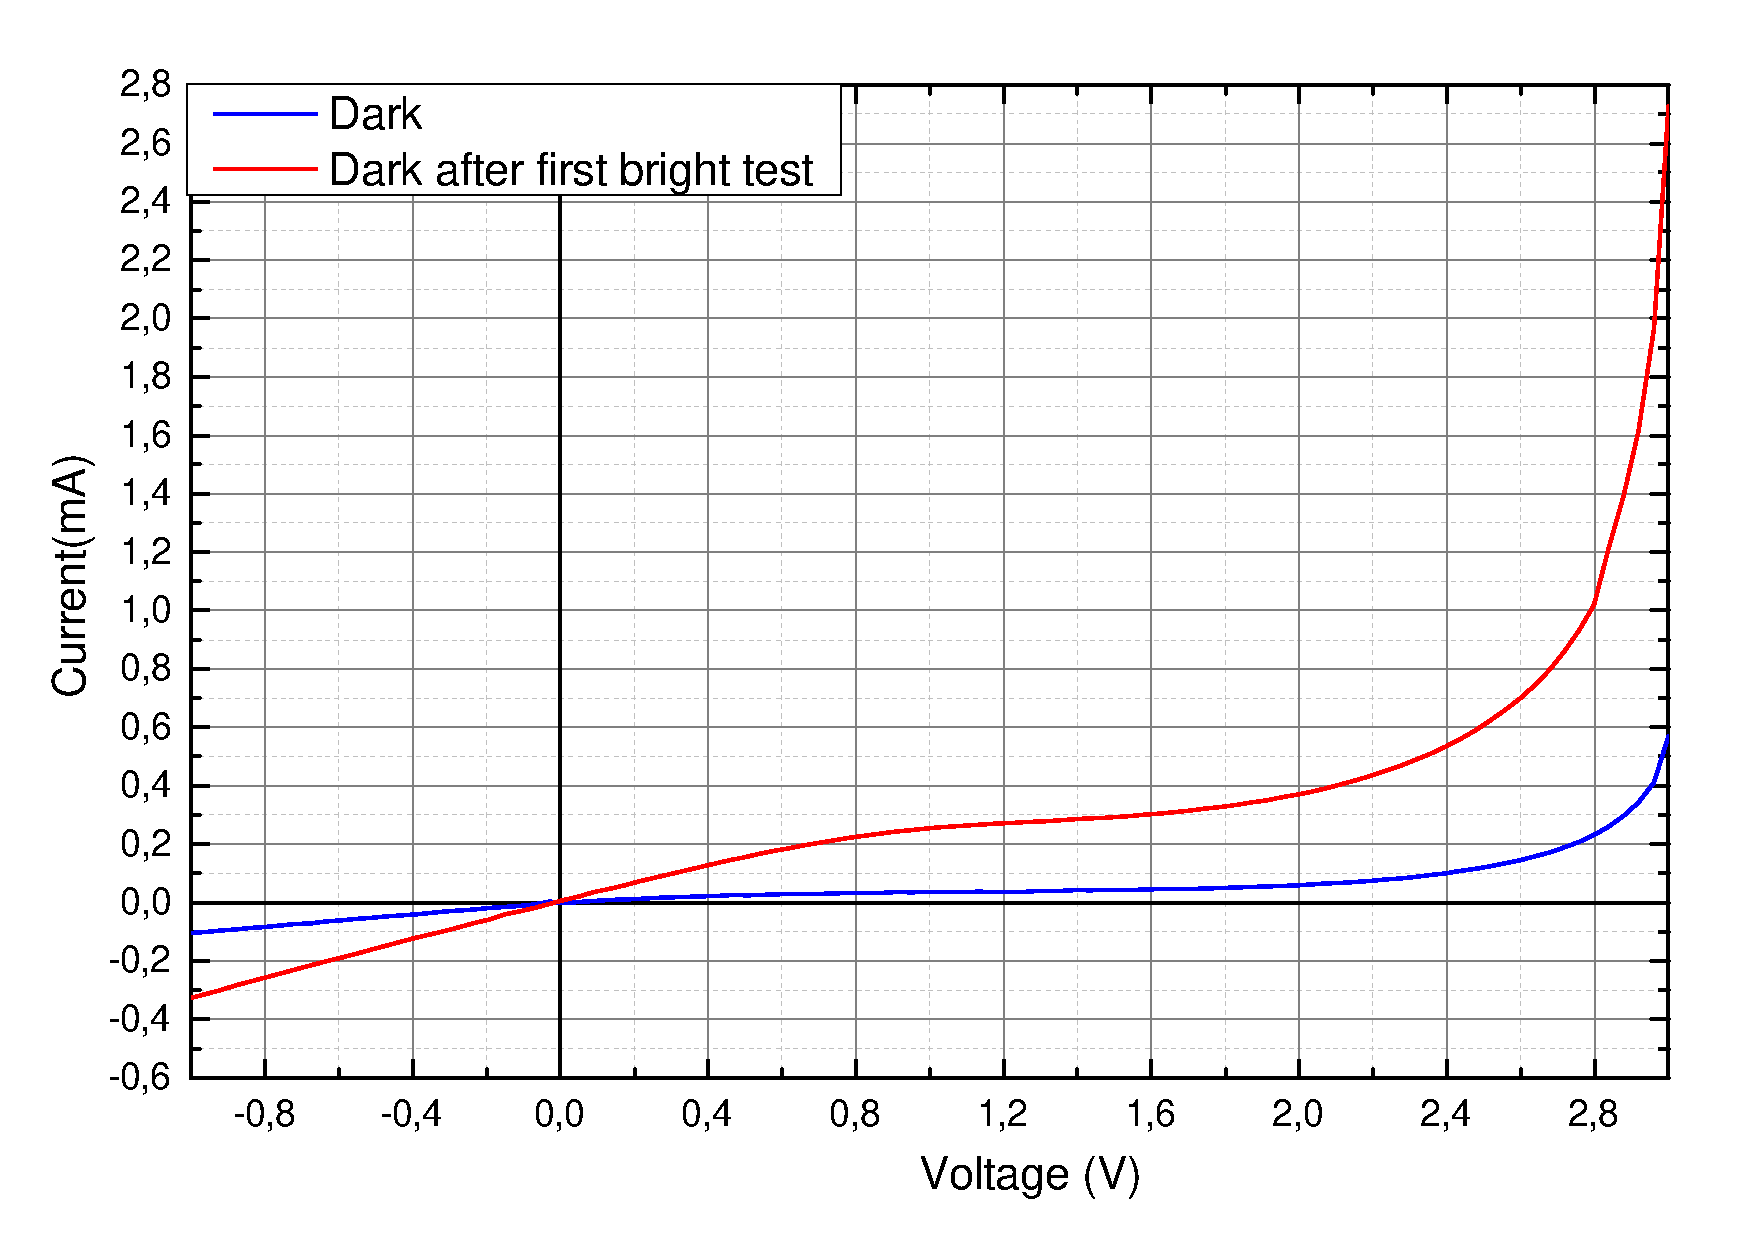
\includegraphics[width = \textwidth]{ch5/Dark}
\caption{Dark spectrum measured for the second time and after one test with bright spectrum}
\end{subfigure}

\hfill

\begin{subfigure}[b]{0.83\textwidth}
\centering
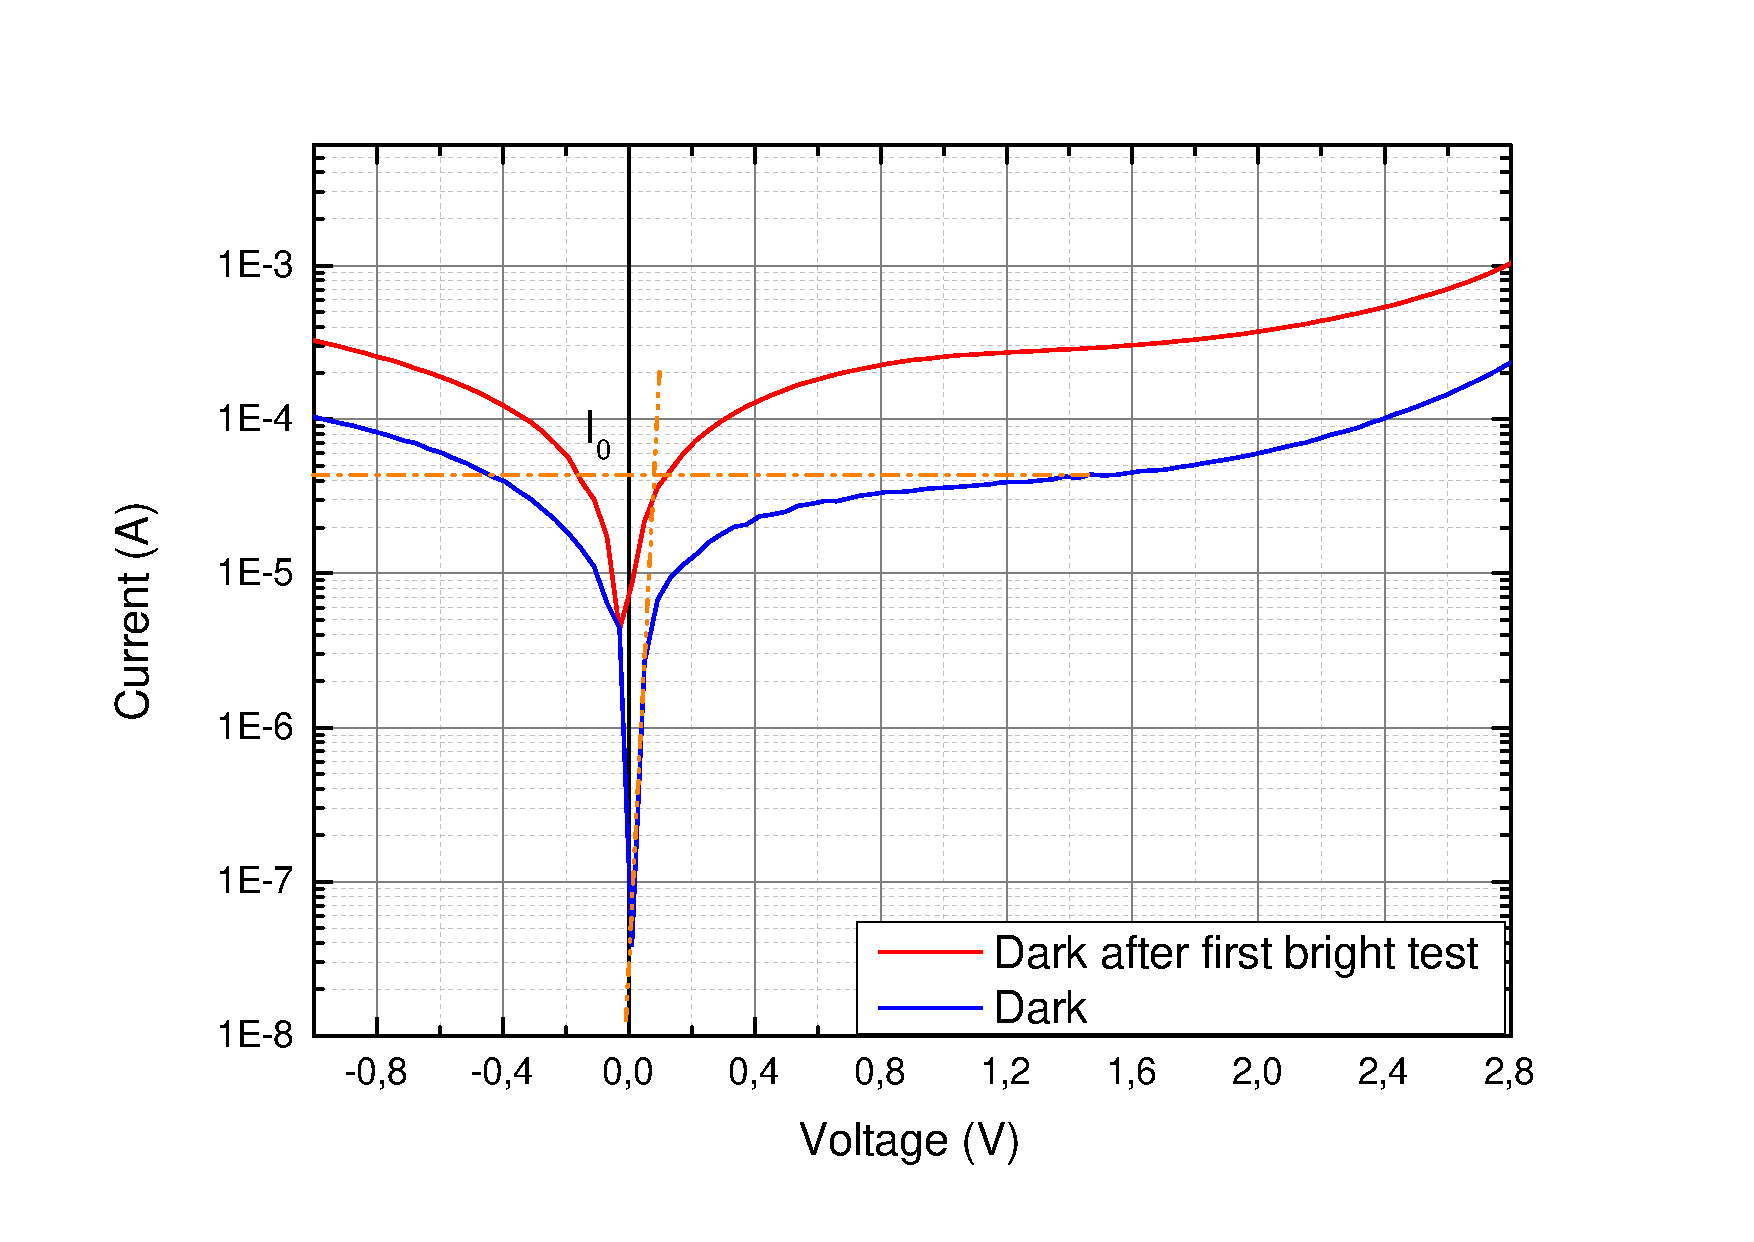
\includegraphics[width = \textwidth]{ch5/Logarithmic Dark}
\caption{Dark spectrum in logarithmic scale}
\end{subfigure}

\caption{Dark IV graph for the second device}
\label{fig:dark}
\end{figure}

After that, the verification of the destruction assumption has been tested. The conclusion is that the device hasn't been destructed completely, yet the beginning of the scope of forward current moved further in the voltage axis and the reverse current again behaved like Ohm-like characteristics. After that, we have checked the bright IV characteristics, with the power of three times the Sun, and the rather surprising results are shown in (Fig.\ref{fig:bright}). To test how the lifetime of the device outlines, we have also shined at it for few minutes and tested the characteristics again. This, unfortunately, has destructed the device completely and I'm afraid this means that it's lifetime is rather scant. On the (Fig.\ref{fig:bright}) we can see 3 tests for bright characteristics and one after the destruction. 

\begin{figure}
\centering
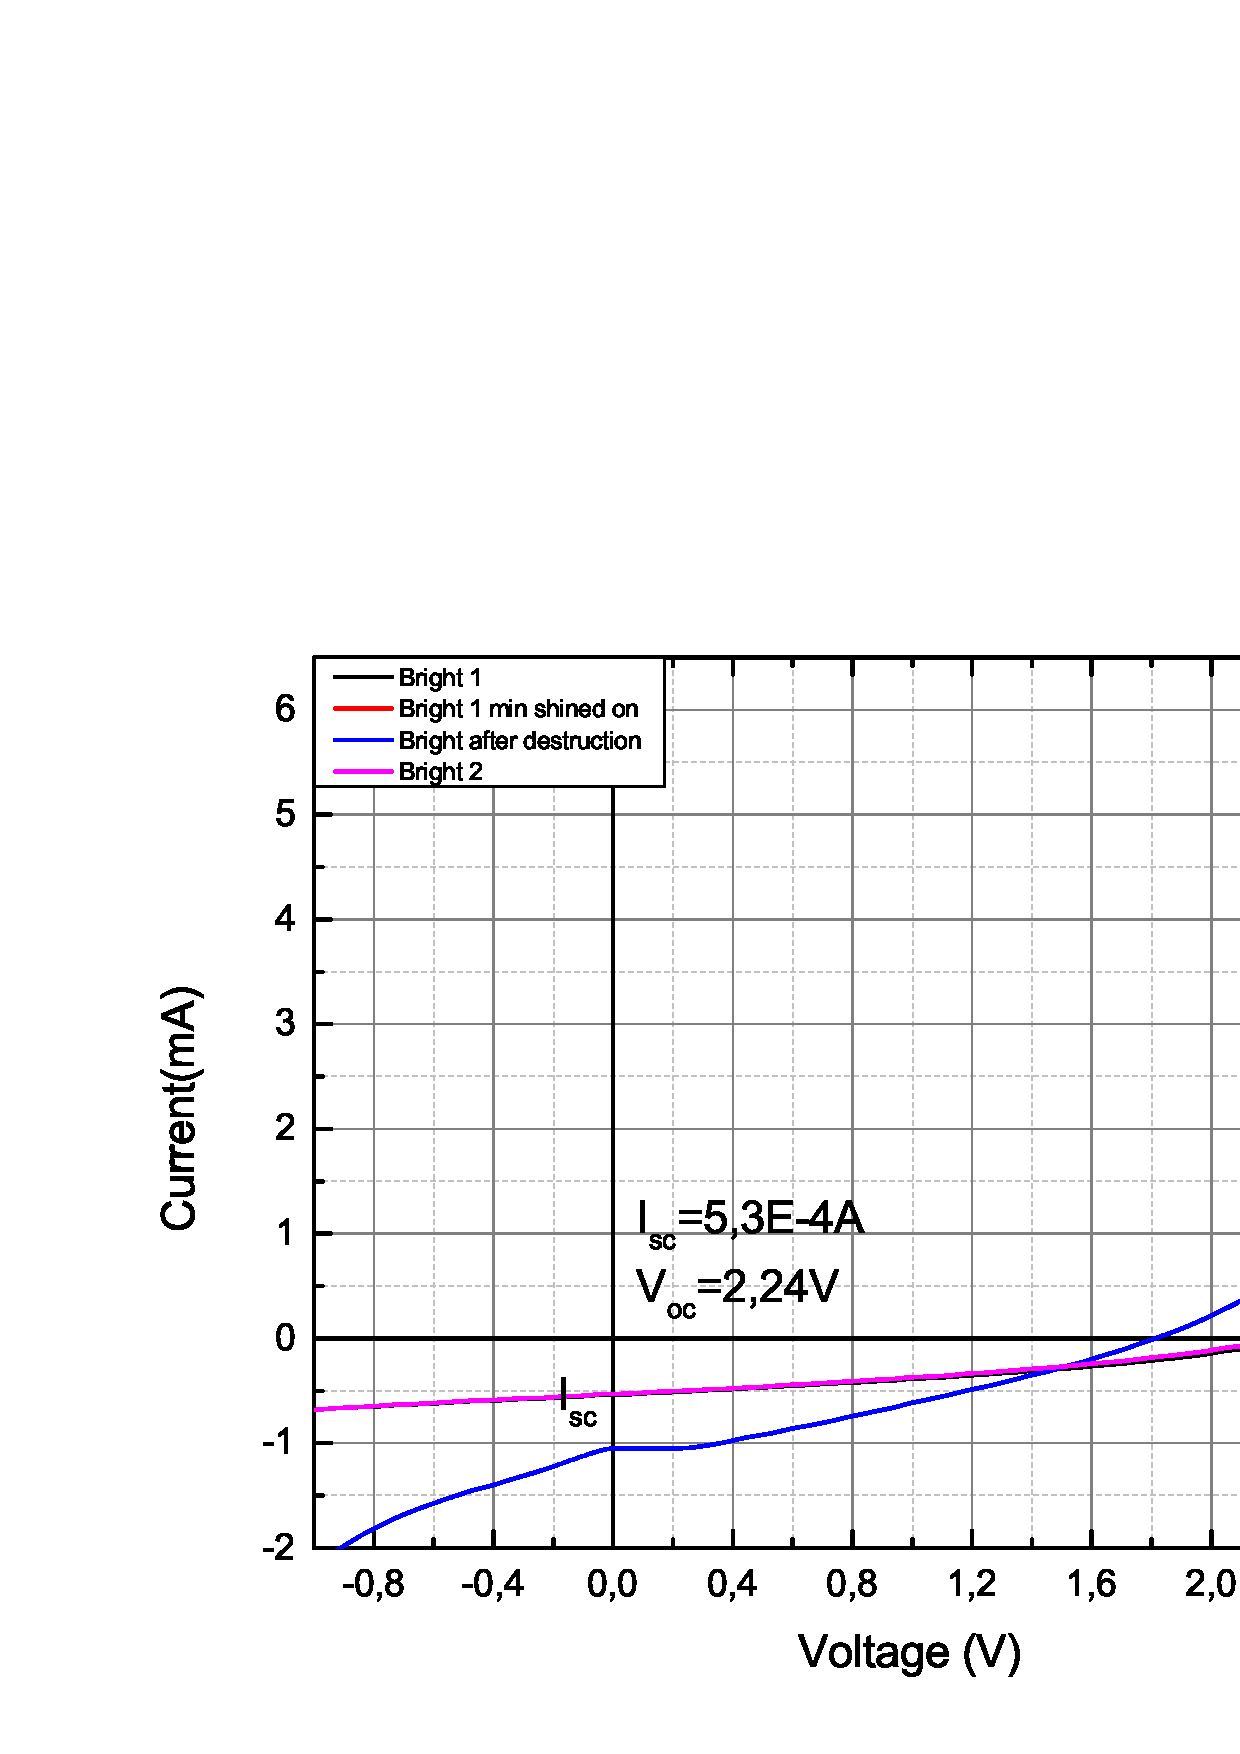
\includegraphics[width = 0.92\textwidth]{ch5/Graph6}
\caption{Bright IV characteristics. Note that the destructed device characteristics is not used(weird things begin to happen there) and the values displayed are for the first test}
\label{fig:bright}
\end{figure}

From those figures we can see that the bright spectrum shows a rather flat but long trend. This means that the \textit{Filling factor} will be small. The short-circuit current is $I_{sc} \approx 0,53mA$ and open-circuit voltage is $V_{oc} \approx 2,24V$. From that we can draw the power graph as well (Fig.\ref{fig:power}). It is crucial to provide the quantities to describe the device. Those are provided below in comparison table.

\begin{table}[b]
\centering
\begin{tabular}{|c |c |c | c | c| c | c | c |}
\hline
& V\textsubscript{m}{[}V{]} & I\textsubscript{m}{[}A{]} &P\textsubscript{in}{[}W{]} & PCE & $V_{oc}[V]$ & $I_{sc}[A]$ & FF\\
\hline
QDSC1 & 0,32 & 6E-05 & 5,75E-03 & 0,33$\%$ & 0,51&1E-04&37,35$\%$\\
\hline
Commercial Cell & 1,45 & 7E-05 & 1,53E-03 & 6,65$\%$ & 2,27 & 1,32E-04 &33,90$\%$\\
\hline
QDSC2 & 1,42 & 3,08E-04 & 5,75E-03 & \textbf{7,62$\%$} & 2,24 & 5,32E-04 &36,78$\%$\\
\hline

\end{tabular}
\caption{Comparison of all of the solar cells}
\end{table}

\begin{figure}[H]
\centering
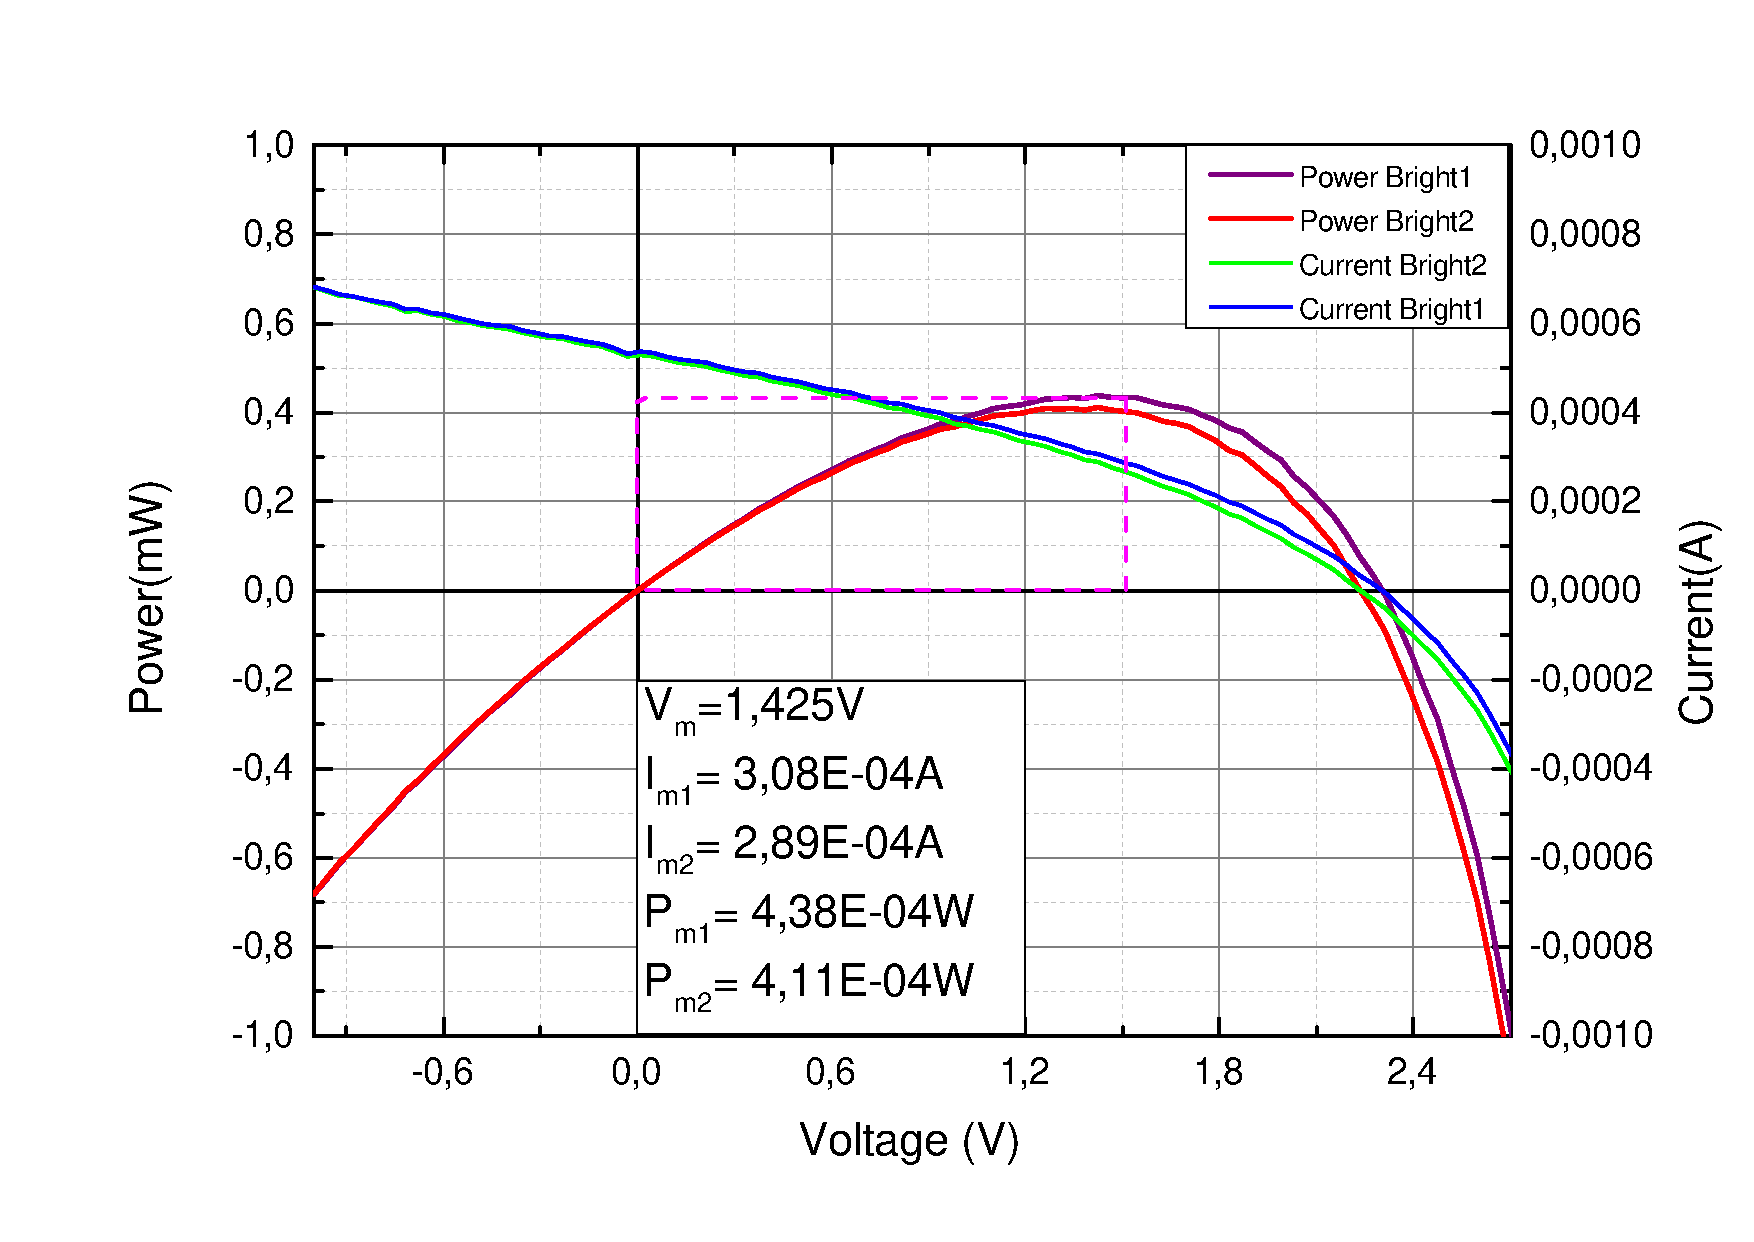
\includegraphics[width = \textwidth]{ch5/Graph3}
\caption{Power plotted for the first and second bright test. Maximal values of are plotted on the graph as well}
\label{fig:power}
\end{figure}

The FF's of the devices were rather similar. Note that, we have stated that the $I_{sc}$ of the former QDSC was really promising but the $V_oc$ is small compared to the commercial device. This is not the case for the second PVD! With even bigger FF and similar $V_{m}$ to Vimun, we have surpassed the device with rank greater $I_m$. This result is really uplifting. From the results above, we can also calculate the shunt and a series resistance if it is to allow us to calculate the generalized current. The shunt resistance can be calculated from the dark IV characteristic, because then you can be sure that no unwanted effects are present and we can achieve real response from material tested. We calculate the shunt resistance as inverse of the scope as $R_{sh}=\left( \frac{dI}{dU}\right) ^{-1}_{U=0}$. Then we can also estimate the series resistance from the semi-logarithmic scale dark IV. It is derived from the deviation of the voltage at current after the exponential dependence isn't that important any more. We have achieved the values for $R_s \approx 2,11 \Omega$ and $R_{sh} \approx 1,44\cdot 10^{4}\Omega$. \cite{Zekry1996}

\begin{figure}[ht]
\centering
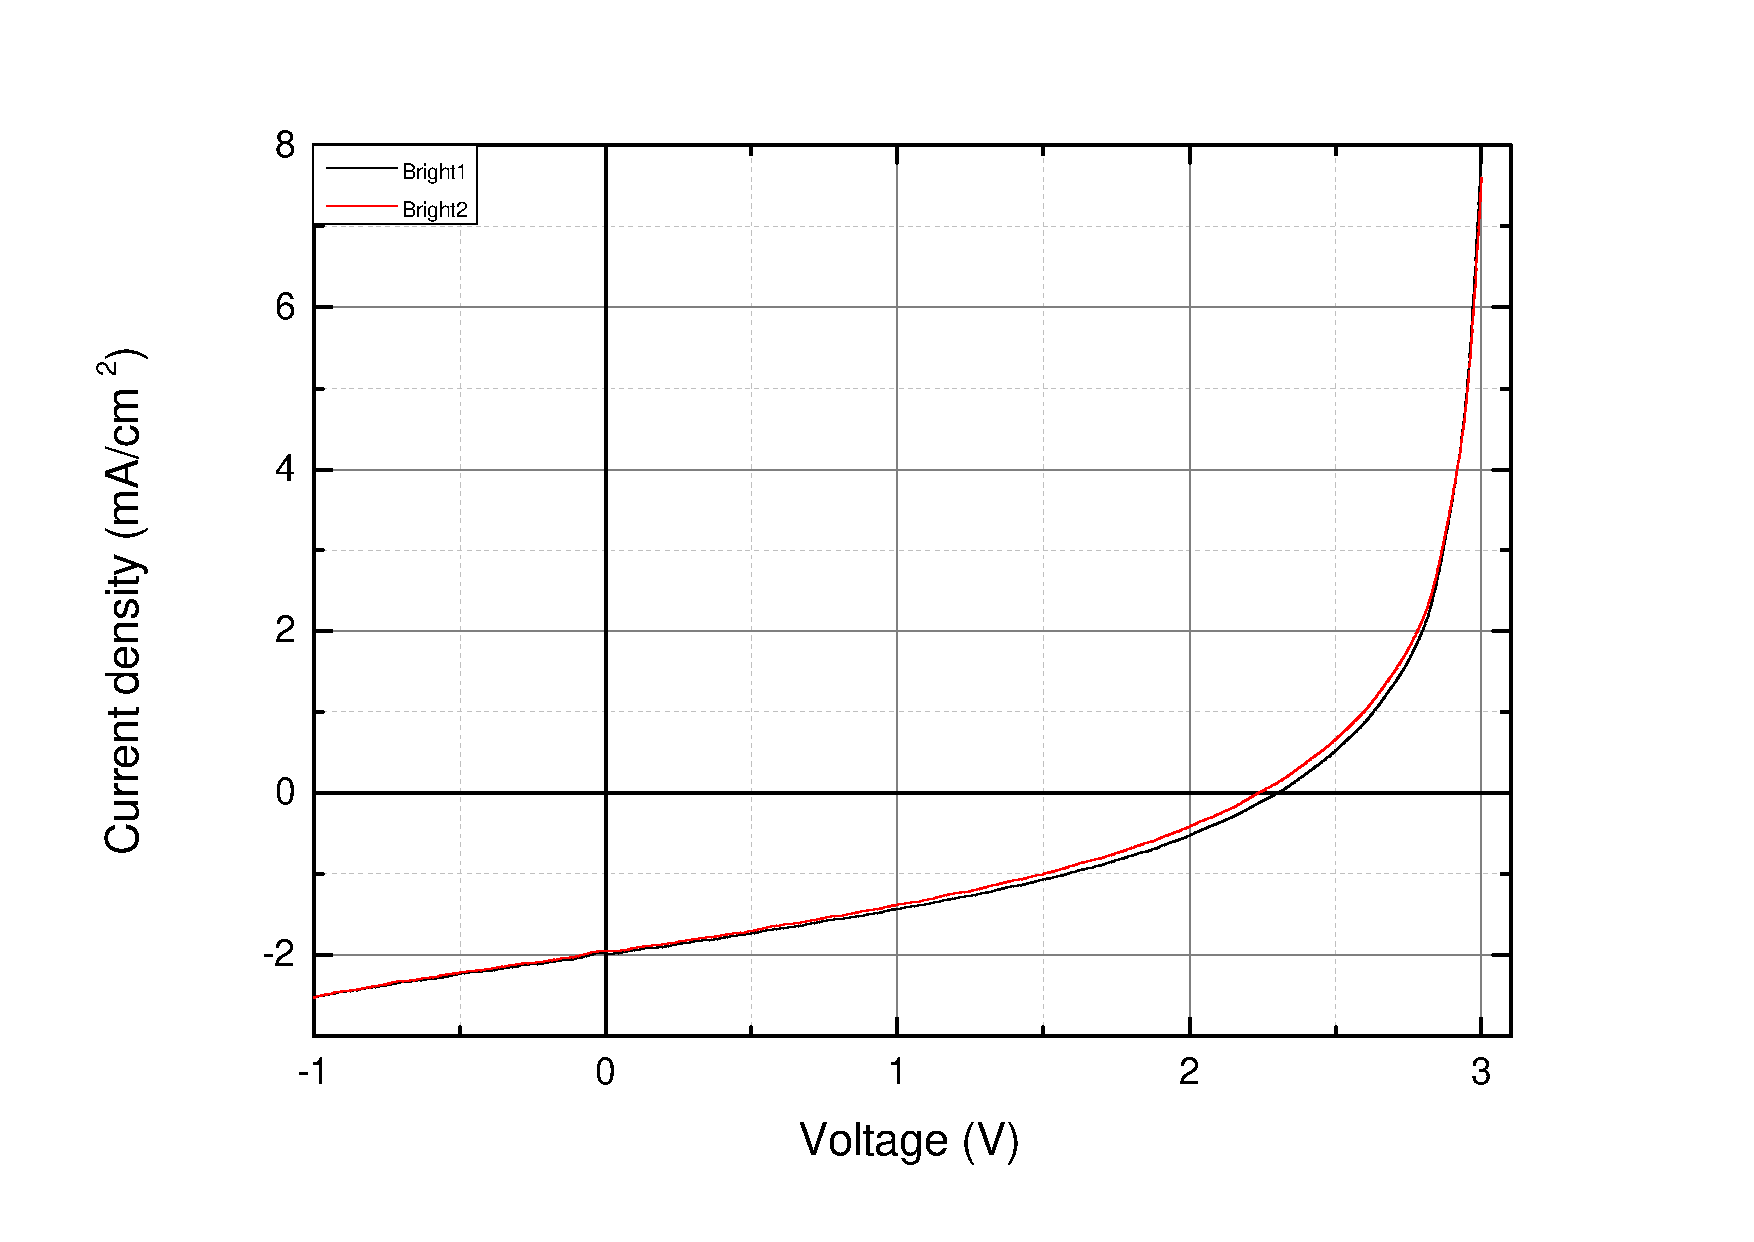
\includegraphics[width = \textwidth]{ch5/Jdens}
\caption{Useful figure for bright characteristics of current density}
\end{figure}
